%-----------------------------------------------------
% Chapter 2: 
%-----------------------------------------------------
\chapter{{Sistemas CAD}}
\label{chap: cap2}
En este capítulo se describen los conceptos generales que involucran la representación de los modelos 3D, la visualización, la manipulación y las características para que puedan aplicarse en la fabricación digital. Al final del capítulo se describen algunos antecedentes de aplicaciones CAD de escritorio y web que incorporan estos conceptos.\newline

\section{Introducción}

La interacción entre el diseñador y el modelo en un proceso de diseño no es una necesidad reciente, de hecho antecede la existencia de la computación. 
Desde principios del siglo XX se registran antecedentes como la maqueta que utilizó el arquitecto Antoni  Gaudí\footnote{\url{http://www.antonigaudi.org/}} para representar el modelo de la cripta de la Colonia Guell\footnote{\url{http://www.gaudicoloniaguell.org/}}, esta se conformaba por  cadenas que sostenían pesos y actuaban por la fuerza de la gravedad \citep{Davis2013}. El modelo fue realizado al revés y se sacó una fotografía para poder visualizarlo al derecho como se puede ver en la figura \ref{fig:gaudi}. 

\begin{figure}[ht]
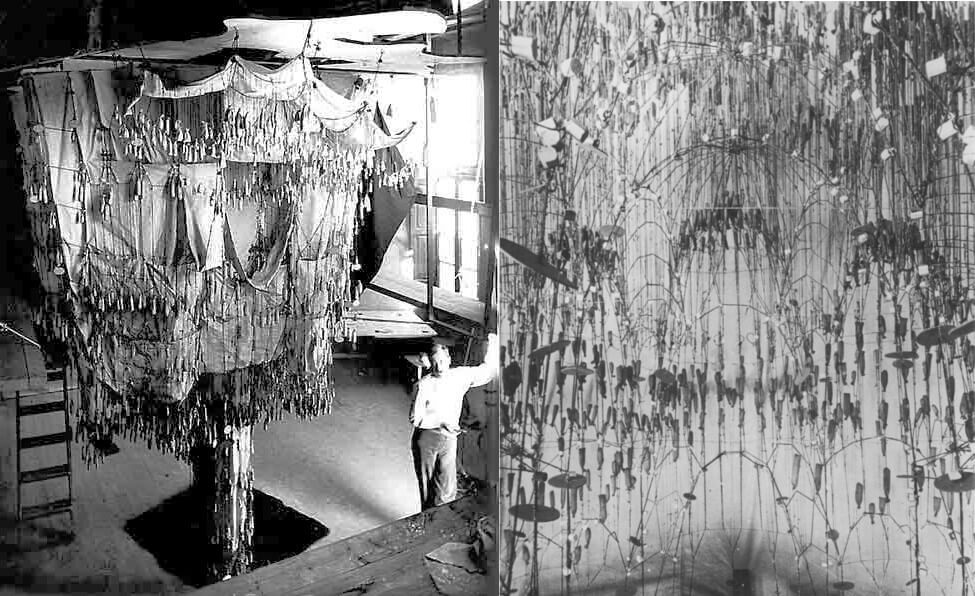
\includegraphics[width=10cm]{Img/GEO/geo-gaudic.jpg}
\centering
\caption{\footnotesize{Maqueta gravitatoria de Gaudí para la cripta de la Colonia Guell. A la derecha una fotografía al revés donde se pueden apreciar los arcos catenarios utilizados para el modelo arquitectónico  \citep{AA.VV2002}.}}
\label{fig:gaudi}
\end{figure}

Una cadena que cuelga tiene por lo menos cuatro parámetros: su longitud, su peso y los dos puntos a los que está sujetada. Al estar colgando por la acción de la fuerza de gravedad adopta una forma curva, definida por la función explicita de los parámetros de la cadena. A pesar de ser análogo, este es un modelo paramétrico debido a la presencia de parámetros que controlan una forma derivada de una función (calculada por la acción de la gravedad). Así, el diseñador puede modificar  un diseño representado por un modelo visual de forma interactiva y en tiempo real, en este caso mediante arcos catenarios\footnote{Una catenaria es una curva ideal que representa físicamente la curva generada por una cadena, cuerda o cable sin rigidez flexional, suspendida de sus dos extremos y sometida a un campo gravitatorio uniforme}.

No fue hasta la aparición de las computadoras y el primer programa CAD, \textbf{Sketchpad} \citep{Sutherland:1963:SMG:1461551.1461591} (ver figura \ref{img:sketchpad}) que se facilitó la interacción en tiempo real del diseñador y la computadora.

\begin{figure}[ht]
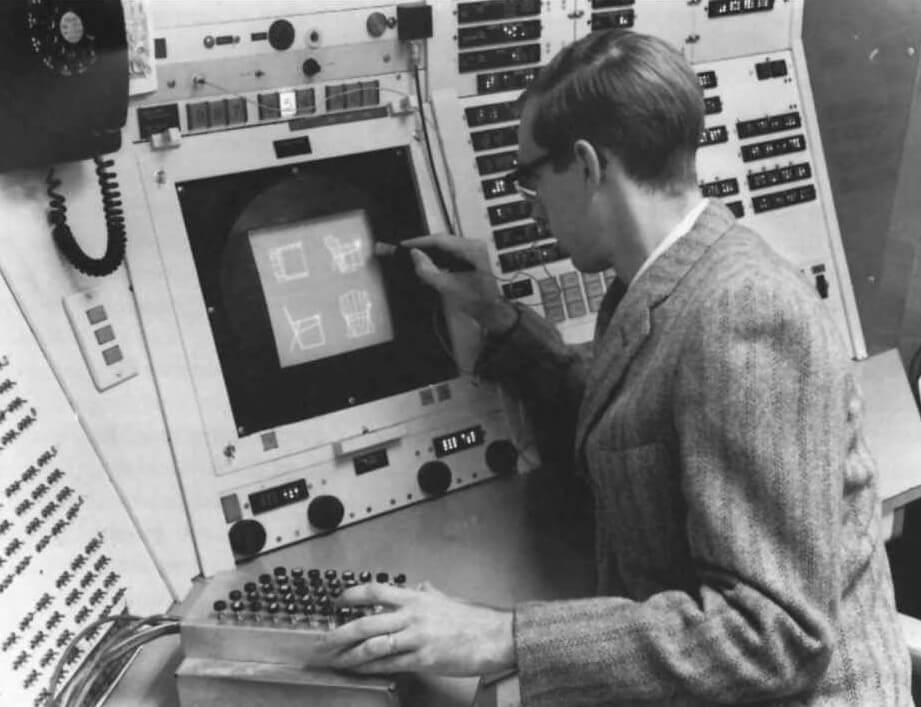
\includegraphics[width=10cm]{Img/GEO/geo-sketchpadc.jpg}
\centering
\caption{\footnotesize{Ivan Sutherland utilizando sketchpad en 1963 \citep{evolved2017}.
}}
\label{img:sketchpad}
\end{figure}



En este contexto, para comprender el uso de tecnologías CAD es fundamental diferenciar  los conceptos  \textbf{computarización del diseño} y  \textbf{diseño computacional}. El primero indica el uso de la computadora como herramienta de dibujo o representación formal orientado a disciplinas creativas, por ejemplo al realizar arte digital\footnote{El arte digital engloba una serie de disciplinas creativas en las que se utilizan tecnologías digitales en el proceso de producción o en su exhibición}, mientras que el diseño computacional aborda el diseño con bases en el pensamiento algorítmico, incluyendo el diseño paramétrico y el generativo \citep{Kaled2016}.



\section{Diseño Paramétrico}
\label{cadparam}
El \textbf{Diseño Paramétrico} se entiende en términos generales como un proceso de descripción de una problemática utilizando variables. Actualmente para describir estas variables, los diseñadores introducen valores o algoritmos en un software especializado como AutoCAD\footnote{\url{https://latinoamerica.autodesk.com/products/autocad/overview}}, al modificar las variables se generan una serie de alternativas de soluciones y según el criterio del diseñador, se obtiene la solución final. El diseño paramétrico en su definición contemporánea es únicamente posible creando un modelo paramétrico y se define como un conjunto de ecuaciones que expresan una geometría explícitamente por medio de funciones definidas por parámetros \citep{burry2012new}. Con la figura \ref{fig:procesopar} se puede analizar el proceso general:

\begin{itemize}
    \item Primero se realiza la abstracción de ideas y los conceptos del diseño. 
    \item A partir de la abstracción se establecen las condiciones geométricas y matemáticas para dar soporte a las ideas iniciales.
    \item Del punto anterior derivan los parámetros y variables necesarios para programar el proceso. 
    \item Finalmente, de la programación se obtiene la representación visual para explorar los resultados. 
\end{itemize}

En todo momento el diseñador puede modificar las condiciones geométricas y matemáticas, los parámetros de la programación y explorar los resultados.

\newline
Mediante el \textbf{diseño iterativo} en inglés \textit{iterative design} \citep{blokdyk2018iterative} se analizan los resultados, se vuelve a trabajar y refinar el modelo diseñado hasta lograr una versión o solución aceptable. 


\begin{figure}[ht]
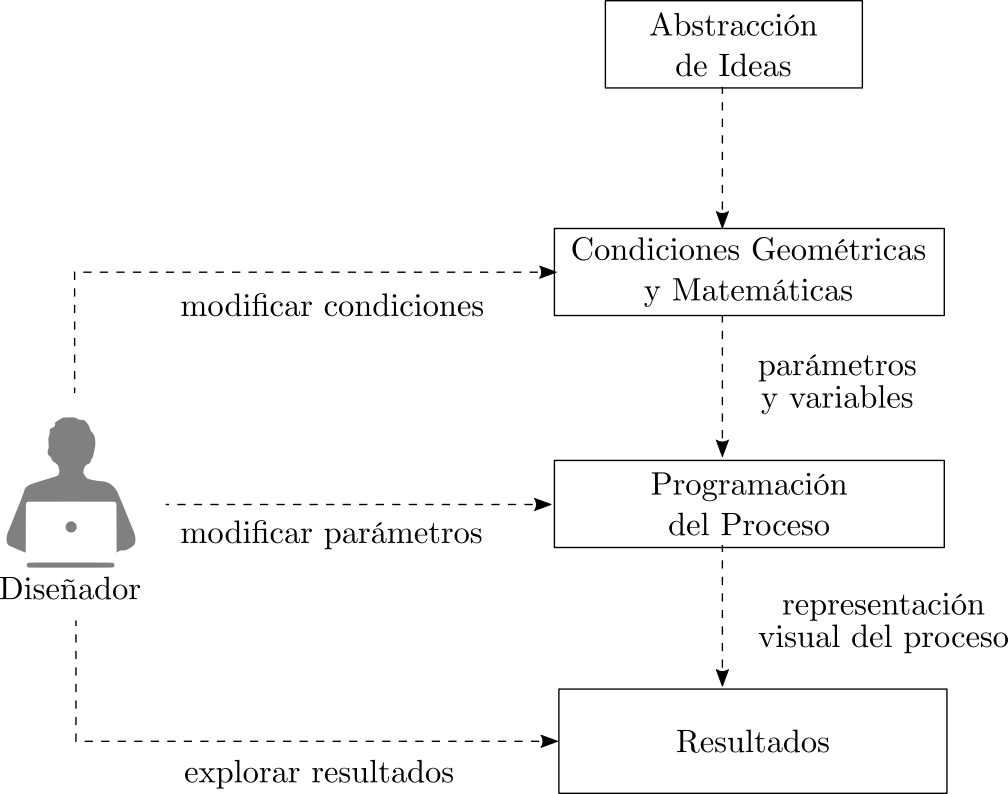
\includegraphics[width=10cm]{Img/CPD/diseno.png}
\centering
\caption{\footnotesize{Proceso general del diseño paramétrico. A partir de la abstracción de ideas y conceptos del diseño se establecen las condiciones geométricas y matemáticas, de estas derivan los parámetros y variables que sirven para programar el proceso, y finalmente de la programación se obtiene la representación visual. En todo momento el diseñador puede modificar las condiciones geométricas y matemáticas, los parámetros de la programación y explorar los resultados. \citep{bohnacker2012generative}.
}}
\label{fig:procesopar}
\end{figure}

Los modelos paramétricos permiten a los diseñadores alterar y modificar la geometría de manera eficiente sin tener que volver a crear el modelo. De esta manera, la parametrización puede elevar la calidad\footnote{{Capacidad que posee un objeto para satisfacer necesidades.}} y la reutilización de un modelo \citep{Alfaiate2017}. Este enfoque de diseño se lleva a la práctica utilizando  \textbf{paquetes aplicativos} o bien mediante la \textbf{codificación por medio de algoritmos}.

\subsection{Diseño paramétrico mediante paquetes aplicativos}

Los paquetes aplicativos de CAD  son aquellos que se instalan en el ordenador y no requieren del uso de internet, como AutoCAD. En este software, el diseño paramétrico se logra utilizando restricciones aplicadas a la geometría \citep{Autodesk2017} y se clasifican en dos tipos: las \textbf{restricciones geométricas} que controlan las relaciones entre los objetos y las \textbf{restricciones por cota} que controlan los valores de distancia, longitud, ángulo y radio de los objetos. Proporcionan una manera de cumplir con ciertos requisitos que permiten  experimentar con los diseños o hacer modificaciones. En el objeto ejemplo de la figura \ref{fig:autocad-0} las modificaciones en un parámetro pueden hacer cambios automáticamente a otros, a la vez se restringe las modificaciones de ciertos valores (como ser distancia y ángulo). Asimismo, las restricciones pueden aumentar su flexibilidad mediante el uso de fórmulas y ecuaciones.


\begin{figure}[ht]
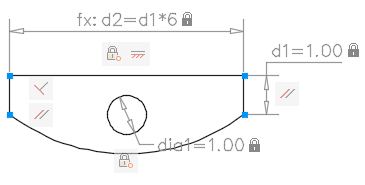
\includegraphics[width=6cm]{Img/CPD/autocad-0.png}
\centering
\caption{\footnotesize{Restricciones en un diseño paramétrico hecho con AutoCAD. Se puede apreciar una restricción mediante la fórmula $d2 = d1*6$ de manera que $d2$ siempre será 6 veces el tamaño de $d1$ (las variables están relacionadas). Por otro lado, el valor del diámetro $dia1$ es independiente a cualquier otra variable. \citep{Autodesk2017}.}}
\label{fig:autocad-0}
\end{figure}

\subsection{Diseño paramétrico especificado en algoritmos} 
\label{dis:script}
 
Las \textbf{interfaces de secuencias de comandos} en inglés \textit{scripting}\footnote{Un script es un programa informático usualmente simple, que por lo general se almacena en un archivo de texto plano. } permiten a los diseñadores/programadores escribir código para automatizar partes del diseño.

El script, con sus parámetros de entrada, funciones explícitas y salidas es una realización arquetípica de la definición matemática de paramétrico \citep{burry2012new}.
Los \textbf{sistemas paramétricos} se basan principalmente en \textbf{principios algorítmicos}, dado que al igual que los algoritmos, toman un valor o un conjunto de valores como entrada, ejecutan una serie de pasos computacionales que transforman la entrada y finalmente producen un valor o un conjunto de valores como salida \citep{Dino2012}. Por lo tanto, las interfaces de scripting disponibles en gran parte de los paquetes CAD están naturalmente predispuestas para generar modelos paramétricos.\newline



\begin{figure}[ht]
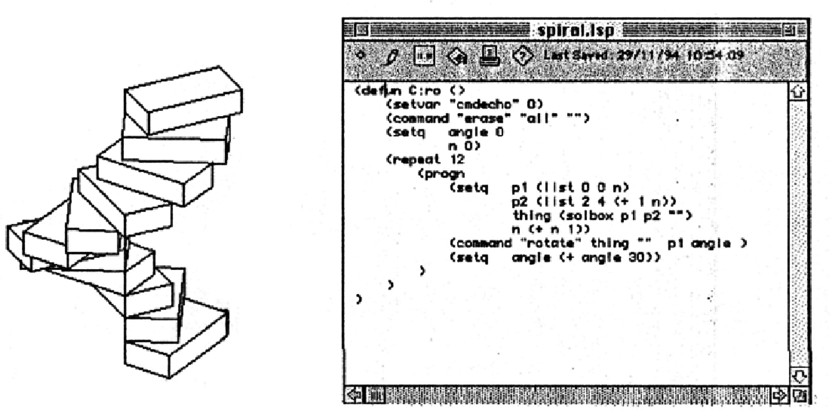
\includegraphics[width=12cm]{Img/CPD/cad-autolisp.jpg}
\centering
\caption{\footnotesize{Programa en código AutoLisp para generar una espiral 3D con bloques simples mediante expresiones anidadas  (derecha). A la izquierda se puede apreciar el modelo resultante del script \citep{Celani2008}.}}
\end{figure}

Independientemente de las aplicaciones que se utilicen para el diseño, los modelos resultantes son útiles para realizar estudios que de otra manera serían difíciles, por ejemplo al no contar con el objeto físico. En este aspecto, entra en juego el \textbf{Modelado Geométrico}  \citep{Ramos2011}, haciendo referencia al conjunto de métodos utilizados para definir la forma y otras características de los objetos. Estos métodos son un compendio de las técnicas utilizadas en varias disciplinas, como la Geometría Analítica y Descriptiva, la Topología, la Teoría de Conjuntos, el Análisis Numérico, las Estructuras de Datos, el Cálculo Vectorial y los Métodos Matriciales. Las aplicaciones de estas técnicas abarcan la \textbf{Representación}, \textbf{Visualización} y \textbf{Diseño} de los objetos.




\section{Modelado Sólido}
\label{ref:modelado-solido}
 El \textbf{Modelado Sólido} \citep{Foley-ITC-1990} es una rama del modelado geométrico que  hace hincapié en la aplicabilidad general de los modelos, e insiste en crear solamente modelos ``completos" de los sólidos, es decir, modelos que son adecuados para responder algorítmicamente (sin la ayuda externa del usuario) a cualquier pregunta geométrica que se formule. Se espera que respondan preguntas geométricas típicas que aparecen en las aplicaciones de ingeniería. Por ejemplo:
¿Cuál es el aspecto del objeto?, ¿Cómo puede fabricarse con los procesos de manufacturación disponibles? 
La respuesta podría ser una imagen, un número o una constante booleana. De hecho, incluso podría ser otro modelo sólido \citep{Ramos2011}. 


\vspace{5mm}
Las \textbf{ventajas prácticas del modelado sólido} son:
\begin{itemize}
    \item Agiliza el desarrollo y los detalles del diseño.
    \item Mejora la visualización y la comunicación del diseño.
    \item Elimina los problemas de interferencias del diseño.
    \item Comprueba la funcionalidad y el rendimiento del diseño (sin la necesidad de prototipos físicos).
    \item \textbf{Proporciona de forma automática las características topológicas para la fabricación digital}, necesarias al programar maquinas herramientas de CNC, impresoras 3D, etc.
\end{itemize}


Un sistema de Modelado Sólido maneja dos tipos de información: los \textbf{datos geométricos} y \textbf{los datos topológicos}. Los datos geométricos son aquellos que representan geométricamente los objetos (coordenadas de vértices, ecuaciones de superficies, etc. En cambio, los topológicos se refieren a cómo conectar componentes geométricos para conseguir un modelo \citep{Ramos2011}.

\subsection{Representación geométrica}
\label{repGeo}

Muchos esquemas de representación y particularmente los modelos sólidos utilizan \textbf{poliedros} \citep{cromwell1999polyhedra} con caras, aristas y vértices.
A bajo nivel, todos los algoritmos que se utilizan se basan en una única primitiva\footnote{Las formas geométricas se denominan  primitivas por su básica constitución en las partes que la conforman.}: el \textbf{polígono}. Internamente los polígonos se dividen en elementos más simples: \textbf{triángulos}.

\begin{figure}[ht]
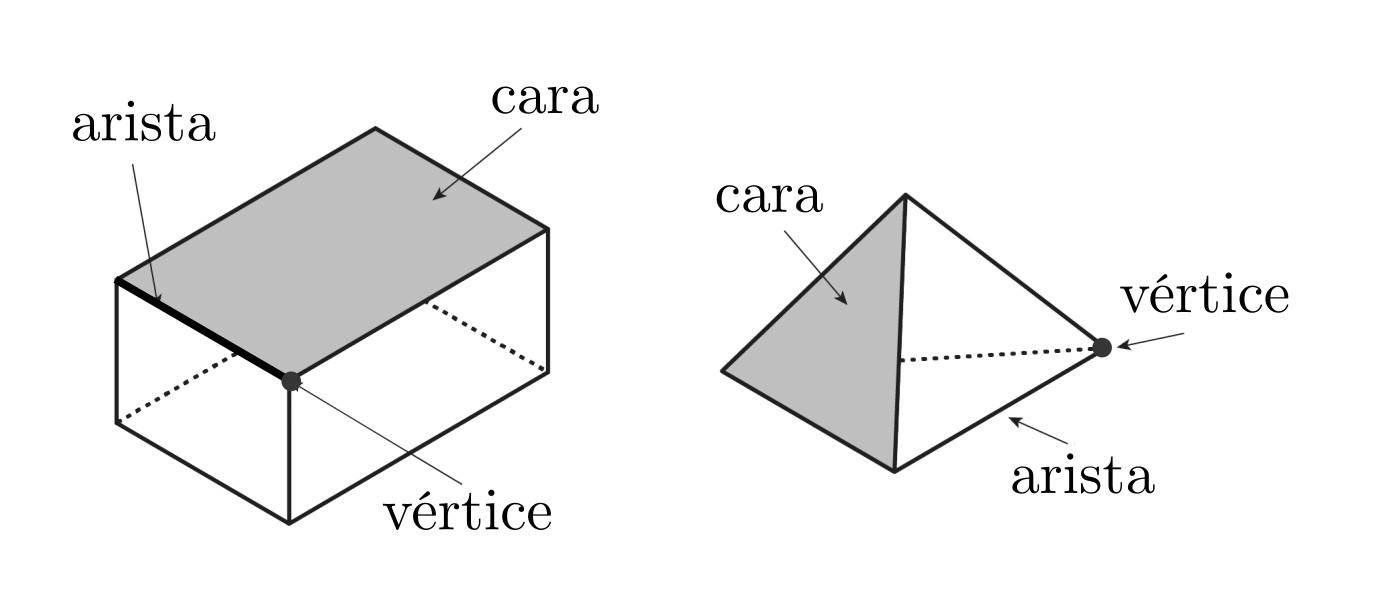
\includegraphics[width=8cm]{Img/GEO/geo-vertex.jpg}
\centering
\caption{\footnotesize{Caras, aristas y vértices en 2 poliedros diferentes: prisma rectangular (izquierda) y tetraedro (derecha).}}
\end{figure}


\subsubsection{Transformaciones 3D}
En términos matemáticos, es común encontrar la representación de los modelos por medio de \textbf{Matrices} \citep{Gabriela2008} (espacio vectorial 3D), estos deben someterse a ciertas transformaciones antes de que su imagen aparezca en la pantalla de un dispositivo. Las transformaciones geométricas se definen como la relaciones de los puntos entre dos imágenes, son operaciones matriciales sobre los puntos del objeto. Cada  objeto se representa como una matriz constituida por las coordenadas (x, y, z) de los puntos que lo conforman  \citep{villamarin2015}.

Las transformaciones básicas son:  \textbf{Traslación  3D}, \textbf{Rotación  3D}, \textbf{Escalamiento  3D} y la composición de las mismas para lograr secuencias de transformaciones.
La traslación mueve un objeto con una trayectoria en línea recta de una posición a otra. La rotación mueve un objeto de una posición a otra a lo largo de una trayectoria circular sobre un eje de rotación específico.


\vspace{5mm}
A modo de ejemplo se explica Escalamiento 3D:

El escalamiento permite cambiar el tamaño de un objeto expandiéndolo o contrayéndolo en sus dimensiones. % \citep{Matias2007}. 
Esto implica el cambio de tamaño de un poliedro, donde cada punto $p = (x,\ y,\ z)$ es transformado por la multiplicación de tres factores de escalamiento: $s_{x}, s_{y}$ y $s_{z}$ a lo largo de los ejes $X,\ Y,\ Z$ respectivamente, de esta forma, las coordenadas del nuevo punto $p^{\prime} = ({x}^{ \prime},\ {y}^{ \prime},\ {z}^{ \prime})$ se obtienen como:
$$
\begin{array}{l@{}l}
{x}^{\prime} = x.s_{x}
\\
{y}^{\prime} = y.s_{y}
\\
{z}^{\prime} = z.s_{z}
\end{array}
$$


Sea $s = (s_{x},\ s_{y},\ s_{z})$ el vector de factores de escalamiento, y $S(s)$ la matriz de
escalamiento, en coordenadas homogéneas \citep{santalo1966geometria} el escalamiento de un punto $p$ en 3D se puede expresar como el producto matricial
$p^{\prime} = p.S(s)$ , es decir:

\begin{equation}
\begin{array}{rccl}
\left[
\begin{array}{rccl}
{x}^{\prime} & {y}^{\prime} & {z}^{\prime} & 1\\
\end{array}
\right]
\end{array}
=
\begin{array}{rccl}
\left[
\begin{array}{rccl}
x & y & z & 1\newline
\end{array}
\right]
\end{array} 
.
\left[
\begin{array}{rccl}
s_{x} & 0 & 0 & 0\\
0 & s_{y} & 0 & 0\\
0 & 0 & s_{z} & 0\\
0 & 0 & 0 & 1\\
\end{array}
\right]   
\end{equation}
\begin{center}
\footnotesize{Expresión matricial para el escalamiento 3D.}
\end{center}

En la figura \ref{fig:escala} se puede apreciar el resultado de un escalamiento con los valores $s_x=2$, $s_y=2.5$ y $s_z=1.5$.

\begin{center}
\begin{figure}[ht]
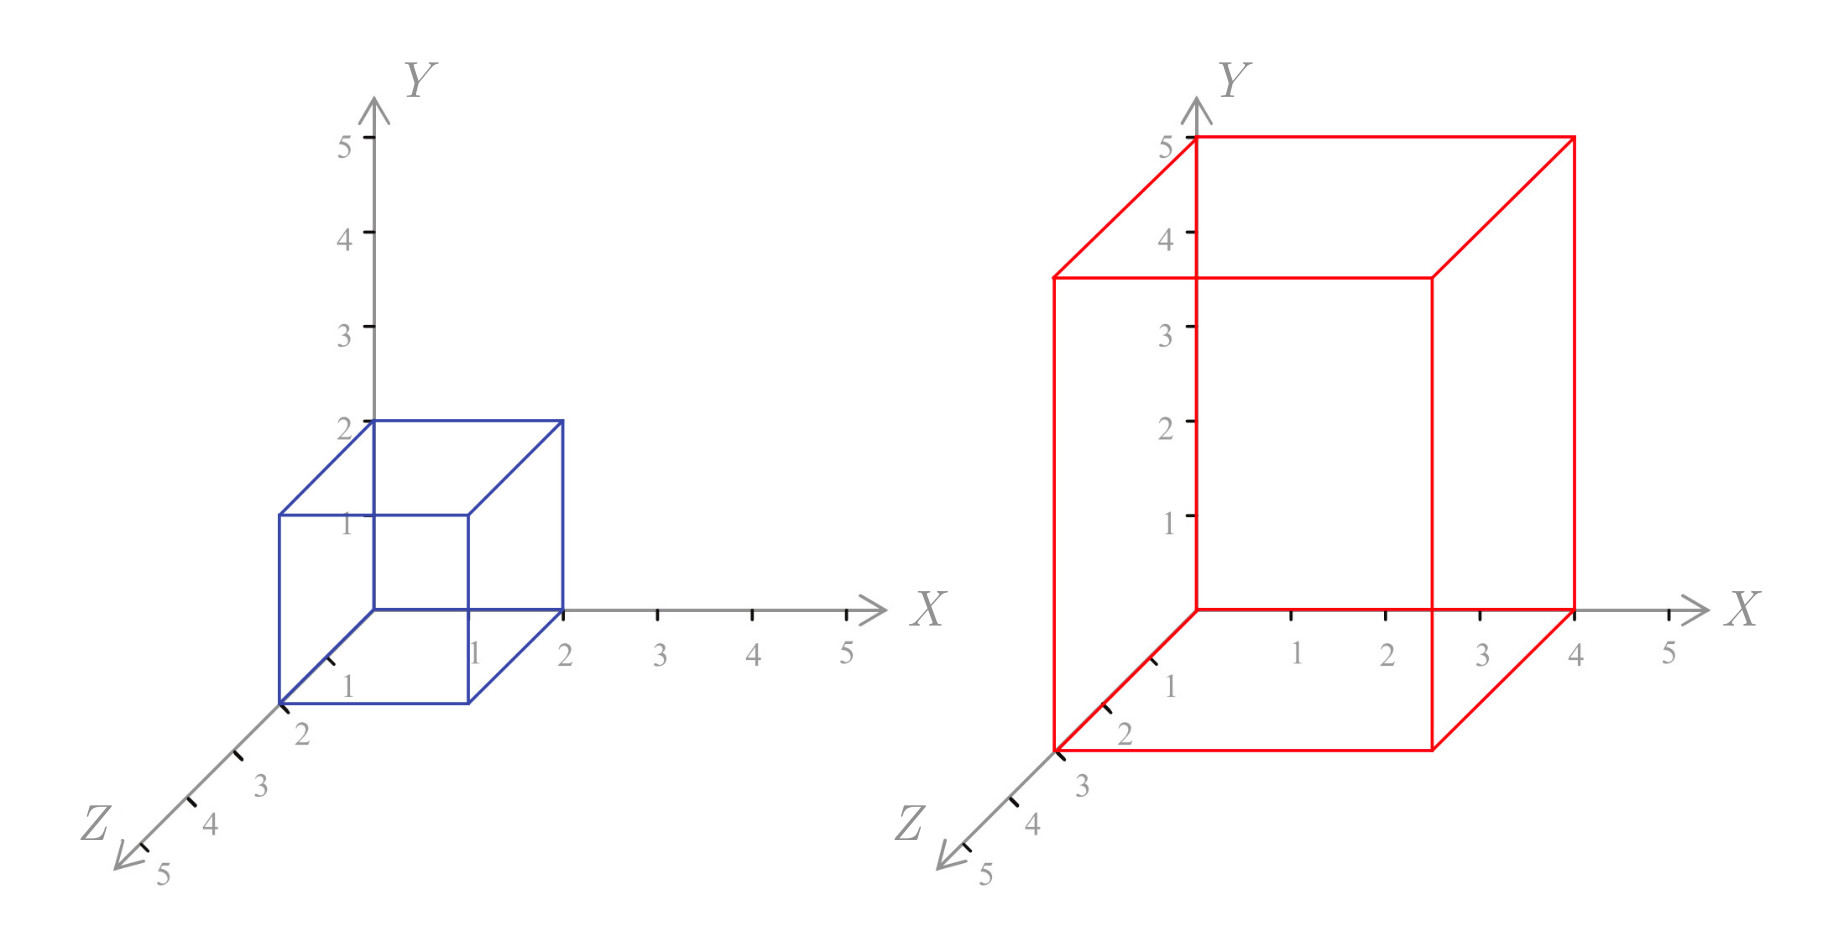
\includegraphics[width=12cm]{Img/GEO/geo-escala0.jpg}
\centering
\caption{\footnotesize{Escalamiento de cubo (izquierda):  aplicando los factores $s_x=2$, $s_y=2.5$ y $s_z=1.5$ se obtiene el objeto de la derecha. Al aplicar diferentes factores se produce una variación en las proporciones del objeto original. \citep{Matias2007}.}}
\label{fig:escala}
\end{figure}
\end{center}


El \textbf{visor} o cámara puede ser considerado como un objeto más, respecto a las transformaciones lineales. Sin embargo, el movimiento de los visores tiene sus propias peculiaridades, por lo que conviene estudiar de modo independiente las transformaciones lineales que se aplican a estos objetos. Por ejemplo: El cambio de escala en el visor produce el efecto zoom (acercar/alejar) \citep{Ramos2011}.

\subsubsection{Topología de los modelos sólidos}
\newline
Conocer las características topológicas de los poliedros es importante para la construcción de los modelos sólidos y especialmente para su validación. 

Los sólidos están definidos en el espacio Euclídeo $E^3$, ocupando una determinada porción de ese espacio. Por lo tanto, se considera un sólido como un conjunto de $E^3$. Obviamente no todos los subconjuntos del espacio Euclídeo son sólidos (por ejemplo un punto aislado no es un sólido). Para que un conjunto de puntos represente un sólido a nivel abstracto,  deberá satisfacer las siguientes condiciones \citep{Torres2014}:

\begin{itemize}
    \item \textbf{Ser cerrado y acotado}. 
    Esto significa que contiene a su frontera (o borde) y ocupa una porción finita del espacio.
    \item \textbf{Ser rígido}. Los sólidos no se modifican al trasladarlos o rotarlos. O lo que es lo mismo, dos sólidos que se diferencian tan solo en una transformación son el mismo sólido.
    \item \textbf{Tener Homogeneidad tridimensional}. El sólido debe ser tridimensional en todos sus puntos, es decir, en cualquier punto de él debe ser posible en tres direcciones ortogonales.
\end{itemize}



\begin{figure}[ht]
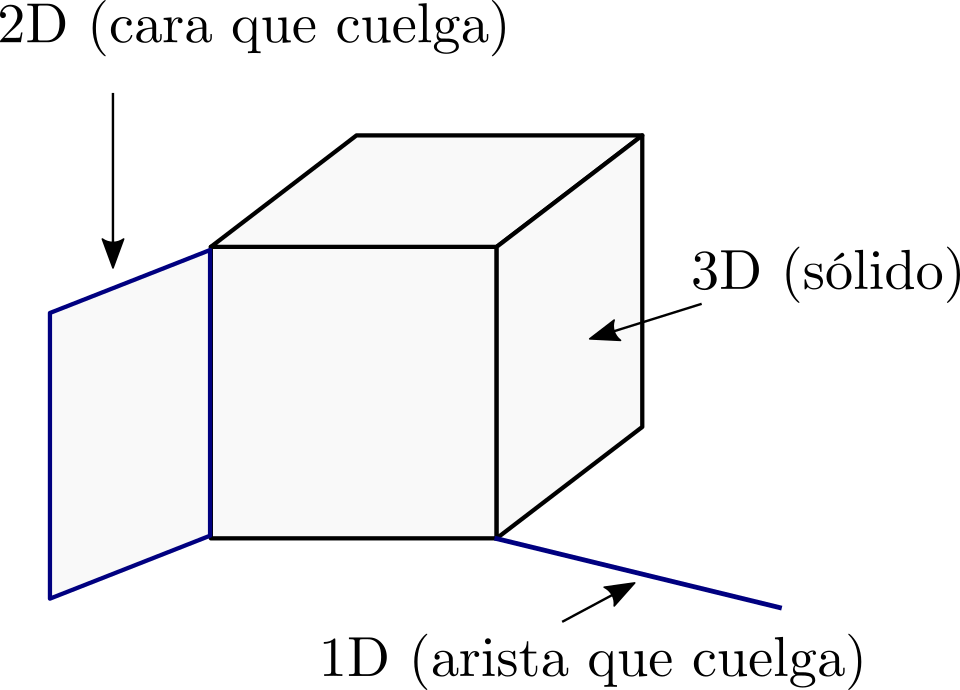
\includegraphics[width=6cm]{Img/GEO/geo-noregular.png}
\centering
\caption{\footnotesize{Objeto que no tiene homogeneidad tridimensional (no sólido). Contiene elementos 2D (cara que cuelga) y 1D (arista que cuelga)  \citep{Torres2014}.}}
\label{fig:geo-noregular}
\end{figure}


A continuación se estudia la topología de algunos poliedros que satisfacen las condiciones para el modelado sólido: Los poliedros simples, no simples y los objetos de Euler.\newline

\subsubsection{Poliedros simples y no simples}\newline
    Un \textbf{poliedro simple} es aquél que puede ser transformado de forma continua en una esfera, o sea, que es topológicamente equivalente a una esfera.

    La \textbf{Fórmula de Euler} para los poliedros simples
    establece que \textquote{\textit{para un poliedro simple se cumple que el número de vértices $V$, menos el número de aristas $A$, más el número de caras $C$}} \citet{Ramos2011} es igual a 2, es decir:

    \begin{equation}
    V - A  +  C = 2
    \label{ec:euler0}
    \end{equation}
    
    Los poliedros regulares forman un subconjunto de los poliedros simples, cuya característica principal es que todas sus caras (polígonos) son iguales, según la fórmula anterior se puede demostrar que sólo existen 5 poliedros regulares: tetraedro, hexaedro o cubo, octaedro, dodecaedro e icosaedro.
    
    
Los \textbf{poliedros no simples} son los equivalentes topológicos de cualquier objeto sólido con huecos, por lo que son muy útiles en el Modelado Sólido \citep{Ramos2011}. 

    \begin{figure}[ht]
    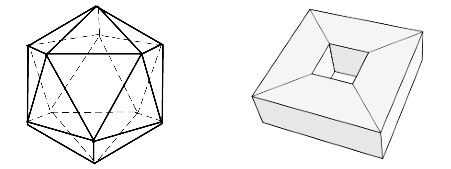
\includegraphics[width=8cm]{Img/GEO/geo-simple-nosimple.png}
    \centering
    \caption{\footnotesize{A la izquierda un poliedro simple regular (icosaedro): se puede transformar en una esfera. A la derecha un poliedro no simple (contiene un hueco): no se puede transformar en una esfera, pero sí en un toro.}}
    \label{fig:polino}
    \end{figure}
    
    Para clasificar los poliedros se recurre al concepto de \textbf{número de conectividad}  (n). Si la superficie de un poliedro se puede dividir en dos regiones separadas mediante un camino cerrado trazado a lo largo de sus aristas, se dice que tiene conectividad $n = 0$. La esfera es un cuerpo que siempre cumple con esa condición, por ende, cualquier poliedro de conectividad $0$ (simple) puede ser transformado en una esfera. Este fenómeno se aprecia con el icosaedro ilustrado a la izquierda de la figura \ref{fig:polino}. 
    Por otro lado, el objeto de la derecha cuenta con caminos cerrados que no dividen a su superficie en dos partes separadas. A estos poliedros se les asigna un número de conectividad mayor que $0$ y por ende, al contener huecos se los denomina \textbf{no simples}.
    
    Si bien los poliedros simples y no simples son sólidos, la fórmula de Euler establece condiciones necesarias, pero no suficientes para que un objeto sea un poliedro. Se pueden construir objetos que satisfagan la fórmula, pero que no acoten un volumen, sin más que añadir una o más caras o aristas colgantes. \textbf{Se requieren de otras restricciones para garantizar que un objeto sea un sólido}.

\subsubsection{ Objetos de Euler }
 $g$ se conoce como \textbf{orden o grado del objeto} y también como \textbf{orden de la superficie}. Así, una esfera equivale a $g = 0 $, un toro, topológicamente hablando, puede considerarse como una esfera con 1 asa ($g = 1$) y así sucesivamente según la cantidad de huecos que tenga el objeto. En la figura \ref{fig:asas} se puede apreciar 3 objetos diferentes que se representan como \textbf{esferas con asas} ($g = 0$, $g = 1$ y $g = 2$) respectivamente.
 
   \begin{figure}[ht]
    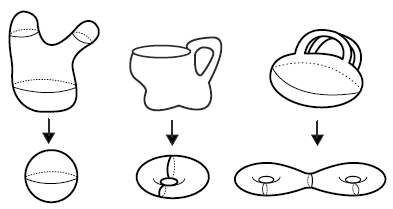
\includegraphics[width=10cm]{Img/GEO/geo-asas.png}
    \centering
    \caption{\footnotesize{Objetos diferentes que se representan como esferas con $g$ asas ($g = 0$, $g = 1$ y $g = 2$) respectivamente. Las asas representan la cantidad de huecos en la superficie de los objetos  \citep{Annenberg}.}}
    \label{fig:asas}
    \end{figure}
 
 Los objetos cerrados tridimensionales de orden $g \geq 0 $ que verifican ciertos requisitos de construcción se denominan \textbf{Objetos de Euler}. Estos requisitos son:
\begin{itemize}
\item Todas sus caras (curvas o planas) han de ser discos topológicos\footnote{Una región, plana o no, que pueda ser transformada en un cuadrado se llama disco topológico y se caracteriza porque no tiene huecos ni puntos aislados en él}, es decir que no tienen huecos ni puntos aislados en ellas. 
\item Cada arista une sólo dos caras y todas finalizan en un vértice en
cada extremo.
\item Como mínimo tres aristas se unen en un vértice. 
\end{itemize}

En todos los objetos de Euler se cumple que:


\begin{equation}
V - A + C  = 2(S-P)
\label{eq:euler1}
\end{equation}

\begin{description}
%\item $A$: Aristas
%\item $C$: Caras
%\item $V$: Vértices
\item $S$: número de superficies inconexas del objeto.
\item $P$: total de pasajes (túneles) en el objeto.
\end{description}

Como el número de pasajes en un objeto es igual al total de ``asas” o agujeros que posea, ocurre que en la ecuación anterior $P$ es igual al orden del objeto $(P = g)$.\newline
Para entender mejor el significado de $S$, la figura \ref{fig:euler} muestra tres objetos eulerianos, con una, dos y tres superficies inconexas.

\begin{figure}[ht]
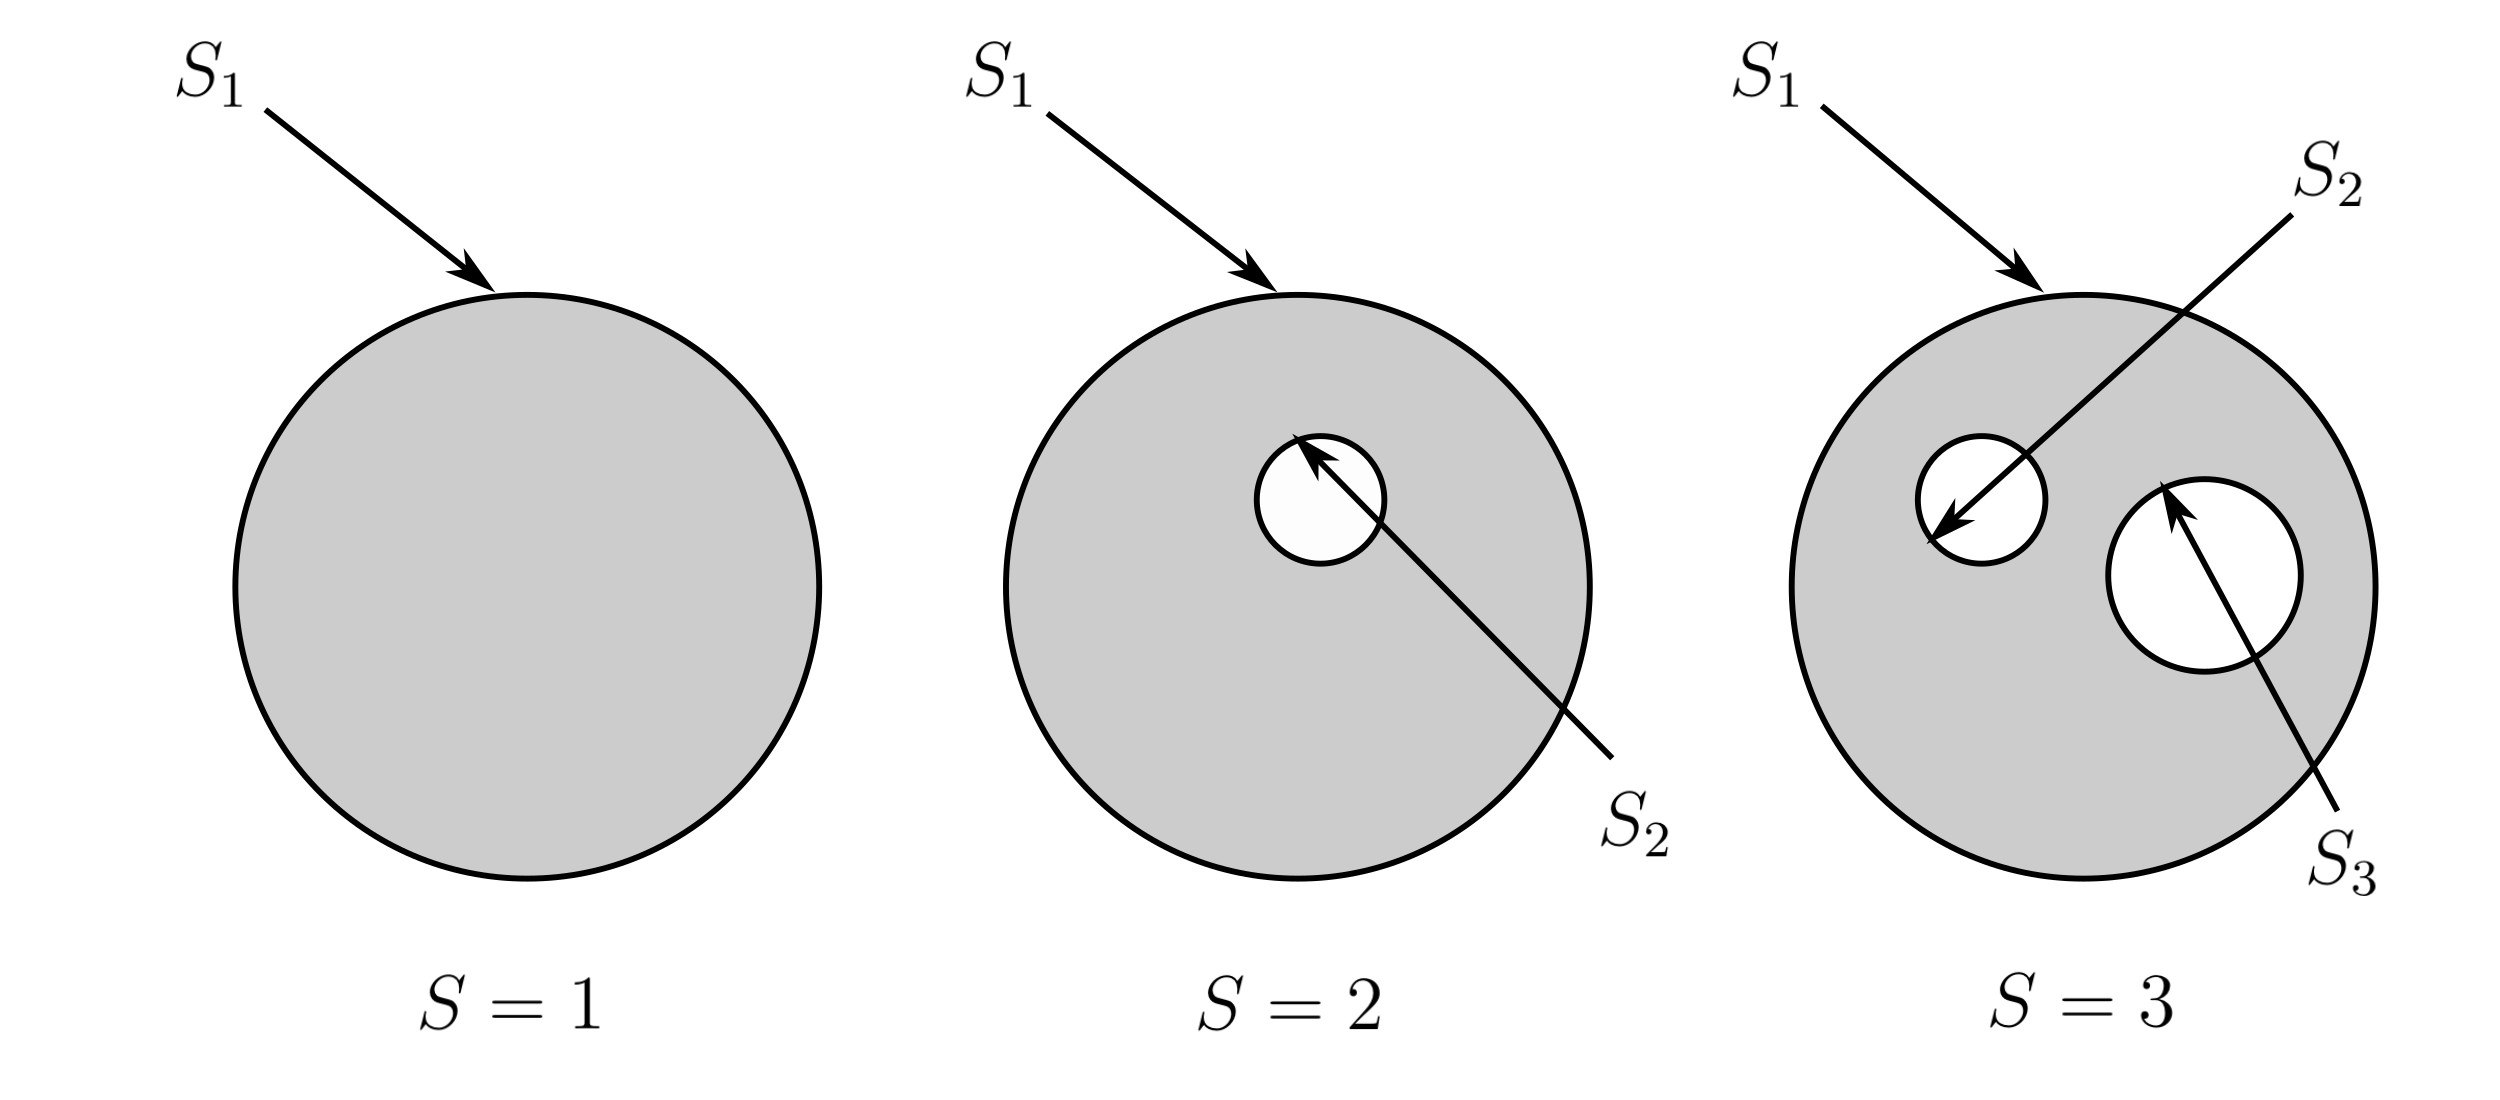
\includegraphics[width=11cm]{Img/GEO/geo-euler0.jpg}
\centering
\caption{\footnotesize{Objetos de Euler con diferentes valores de $S$ (número de superficies inconexas): $S = 1$, $S = 2$ y $S = 3$ respectivamente \citep{Ramos2011}}}
\label{fig:euler}
\end{figure}

En la figura \ref{fig:euler1} se pueden tres ejemplos de objetos eulerianos, a pesar de que cuentan son diferente número de vértices $V$, aristas $A$ y caras $C$, cuando $S = 1$ y $P = 0$ (no poseen huecos) la \ref{eq:euler1} se reduce a la ecuación de Euler para poliedros simples \ref{ec:euler0}. Por ende, estos objetos se representan como poliedros simples.

\begin{figure}[ht]
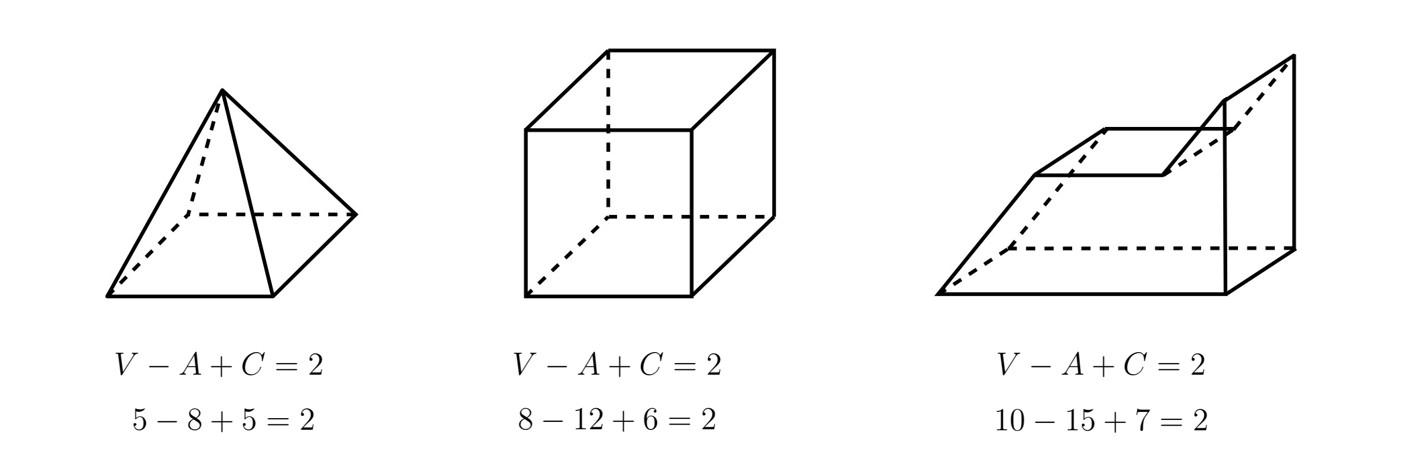
\includegraphics[width=14cm]{Img/GEO/geo-euler1.jpg}
\centering
\caption{\footnotesize{Ejemplos de objetos de Euler con diferentes números de vértices $V$, aristas $A$ y caras $C$. Se puede verificar que en los tres casos se cumple la igualdad. Al no contener huecos se consideran poliedros simples \citep{Ramos2011}.}}
\label{fig:euler1}
\end{figure}


Por otro lado, en la figura \ref{fig:euler2} se ilustran dos objetos de Euler con diferentes $P=0$. 
El objeto de la izquierda, aunque posee una cavidad, esta no llega a atravesar el modelo $P=0$. Por lo tanto, se trata de un objeto sólido topológicamente equivalente a una esfera, es decir, de grado $g = 0$.\newline
Sin embargo, el objeto de la derecha es de grado $g = 1$, ya que tiene un túnel que lo cruza $P=1$ y es un sólido topológicamente equivalente a un toro.\newline


\begin{figure}[ht]
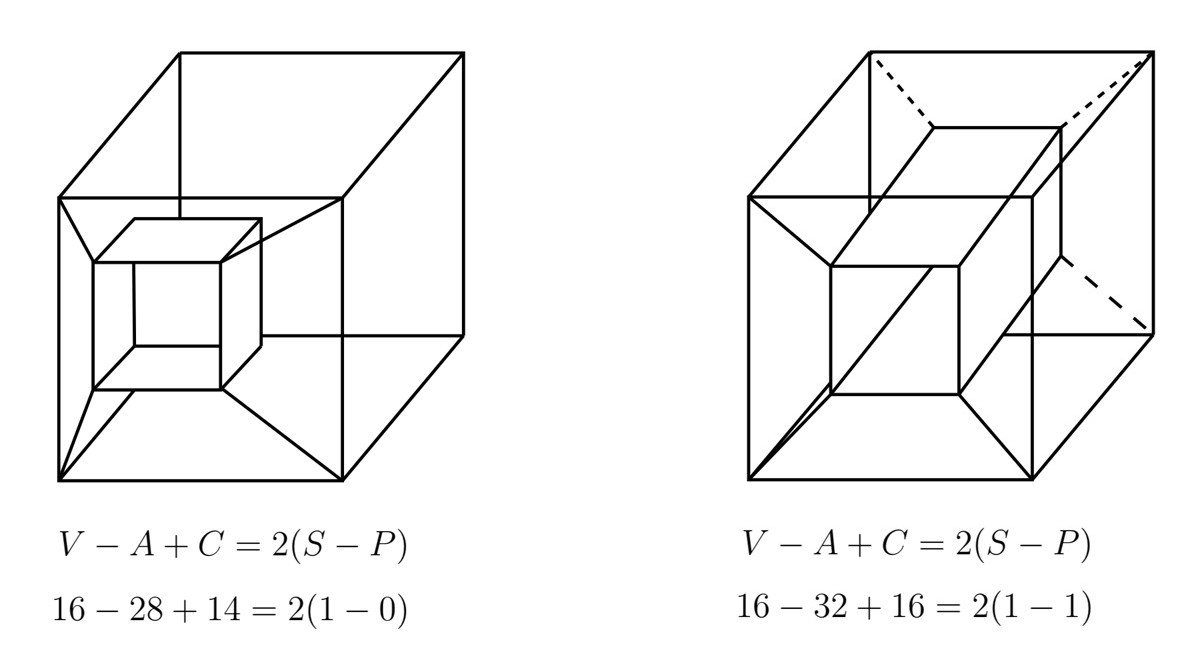
\includegraphics[width=10cm]{Img/GEO/geo-euler2.jpg}
\centering
\caption{\footnotesize{Objetos eulerianos de $g= 0$ y $g=1$, respectivamente. El sólido de la izquierda tiene un túnel que lo atraviesa $P=1$, se puede representar topológicamente como un toro. El de la derecha posee una cavidad, pero esta no llega a atravesar el modelo $P=0$, es un sólido que se puede representar topológicamente como una esfera \cite{Ramos2011}. }}
\label{fig:euler2}
\end{figure}


\subsubsection{Representación por atlas}
Uno de los puntos clave en el modelado con poliedros es cómo se registra su información topológica, es decir, las relaciones entre los vértices, aristas y caras que los definen.
La forma más simple y directa para representar los poliedros consiste en describir cada cara por separado, señalando explícitamente cómo han de unirse. Este método de representación se conoce como \textbf{atlas}. 
La figura \ref{fig:atlascubo} muestra el atlas de un cubo.

\begin{figure}[h]
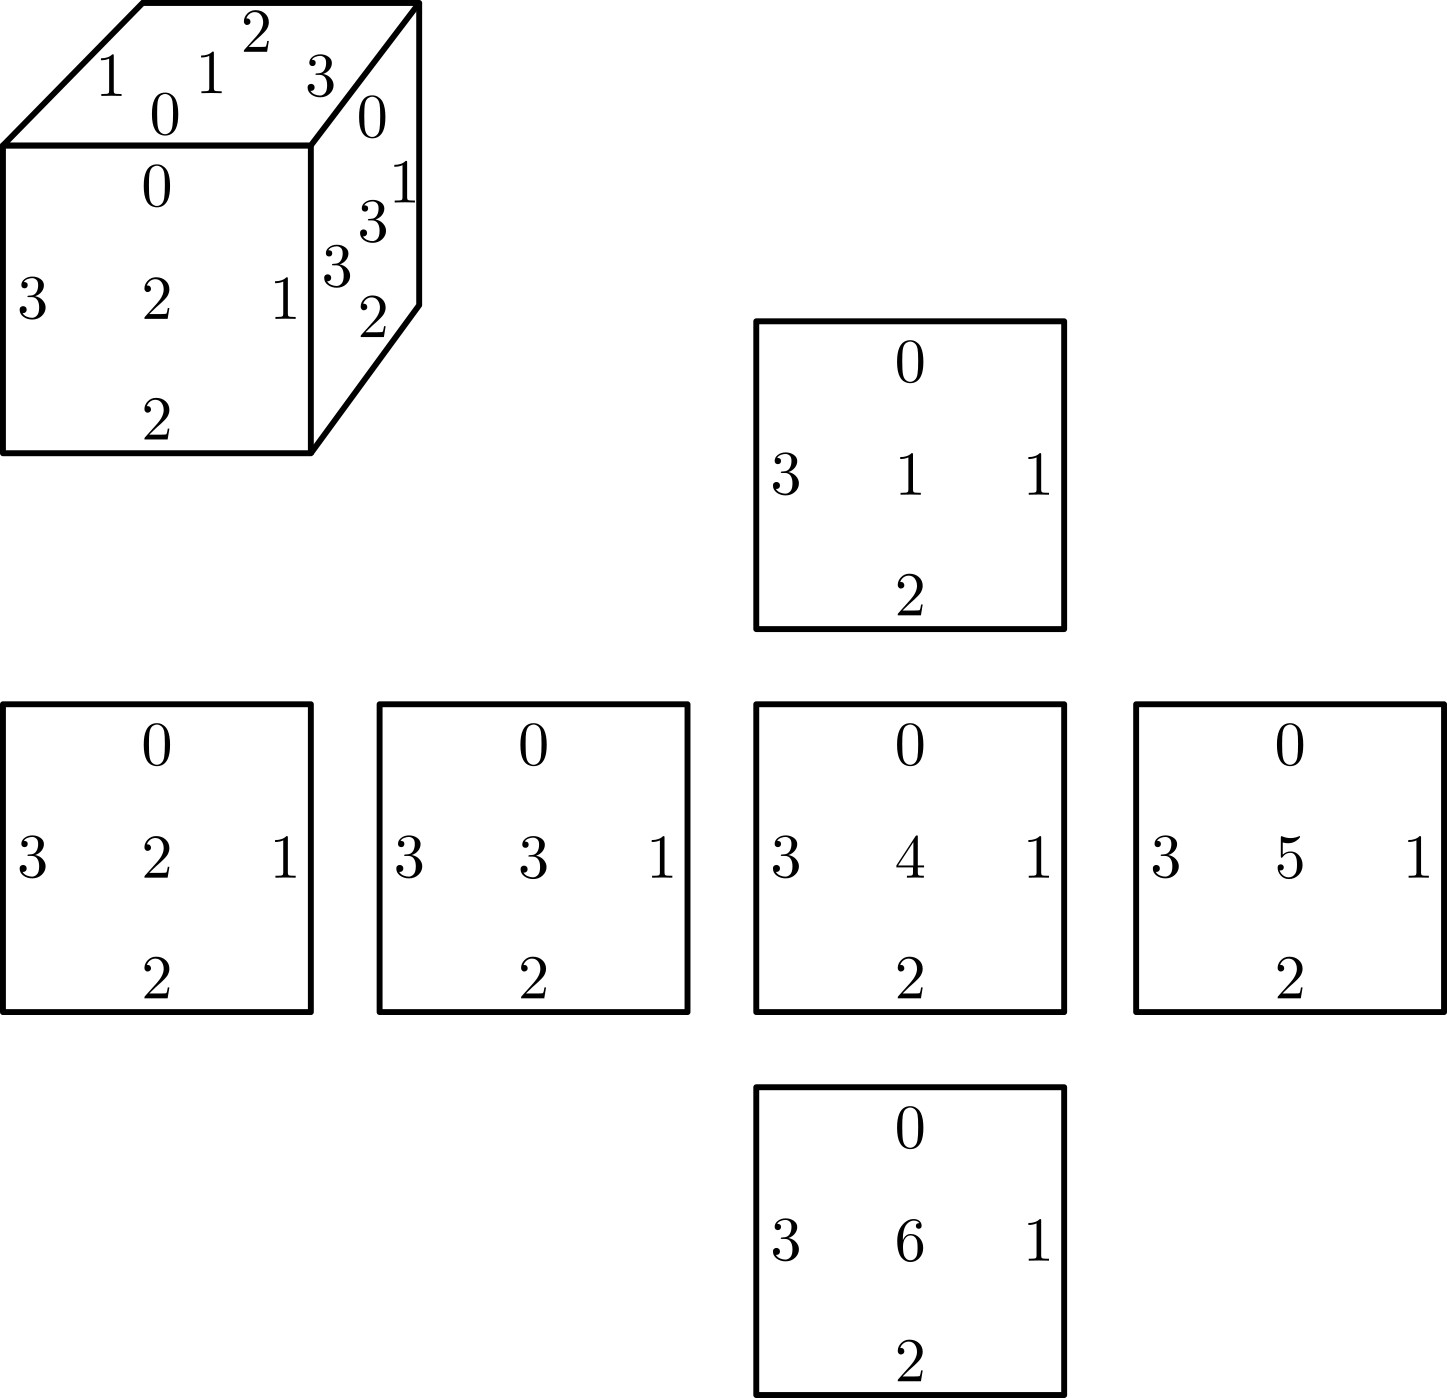
\includegraphics[width=7cm]{Img/GEO/geo-atlas0.jpg}
\centering
\caption{\footnotesize{Atlas de un cubo. El valor del centro indica el número de cara. Los números cercanos al borde indican el número de arista correspondiente a cada cara.
\citep{Ramos2011}.}}
\label{fig:atlascubo}
\end{figure}

Cada eje se etiqueta con un par de números indicando la cara y el número de la arista de la cara. Así el par $(1,\ 0)$ se interpreta como la arista $0$ de la cara $1$. Cada unión de dos aristas se especificará por dos pares de números, identificando las aristas que se unen. De esta forma, el atlas formado queda como:


$$
\begin{array}{c@{}c@{}c@{}c}
 \begin{array}{cc}
         [(1,0) & (2,0)]
  \end{array} & \begin{array}{cc}
         [(1,1) & (5,0)]
  \end{array} & \begin{array}{cc}
         [(1,2) & (4,0)]
  \end{array} &
  \begin{array}{cc}
         [(1,3) & (3,0)] 
  \end{array}
  \\
  \begin{array}{cc}
         [(2,1) & (3,3)]
  \end{array} & \begin{array}{cc}
         [(2,3) & (6,2)]
  \end{array} & \begin{array}{cc}
         [(2,3) & (5,1)] 
  \end{array} &
  \begin{array}{cc}
         [(3,1) & (4,3)]
  \end{array}
  \\
  \begin{array}{cc}
         [(3,2) & (6,3)]
  \end{array} & \begin{array}{cc}
         [(4,1) & (5,3)]
  \end{array} & \begin{array}{cc}
         [(4,2) & (6,0)] 
  \end{array} &
  \begin{array}{cc}
         [(5,2) & (6,1)] 
  \end{array}
\end{array}
$$   

\begin{center}
\footnotesize{Representación matricial del atlas}
\end{center}

Además de especificar qué aristas están unidas, se debe decir cómo unirlas. La figura \ref{fig:atlas0} muestra dos formas diferentes de unir un par de aristas. La primera, mostrada a la izquierda, es la unión con \textbf{orientación conservadora}, y la segunda tiene \textbf{orientación inversora}. Para unir esas dos aristas hay que hacer coincidir los números de cada una de ellas. Si se hace mediante la orientación conservadora se obtiene un cilindro y con la orientación inversora una \textbf{cinta de Moebius}\footnote{La cinta de Möbius o Moebius es una superficie con una sola cara y un solo borde. Tiene la propiedad matemática de ser un objeto no orientable.}.

\begin{figure}[h]
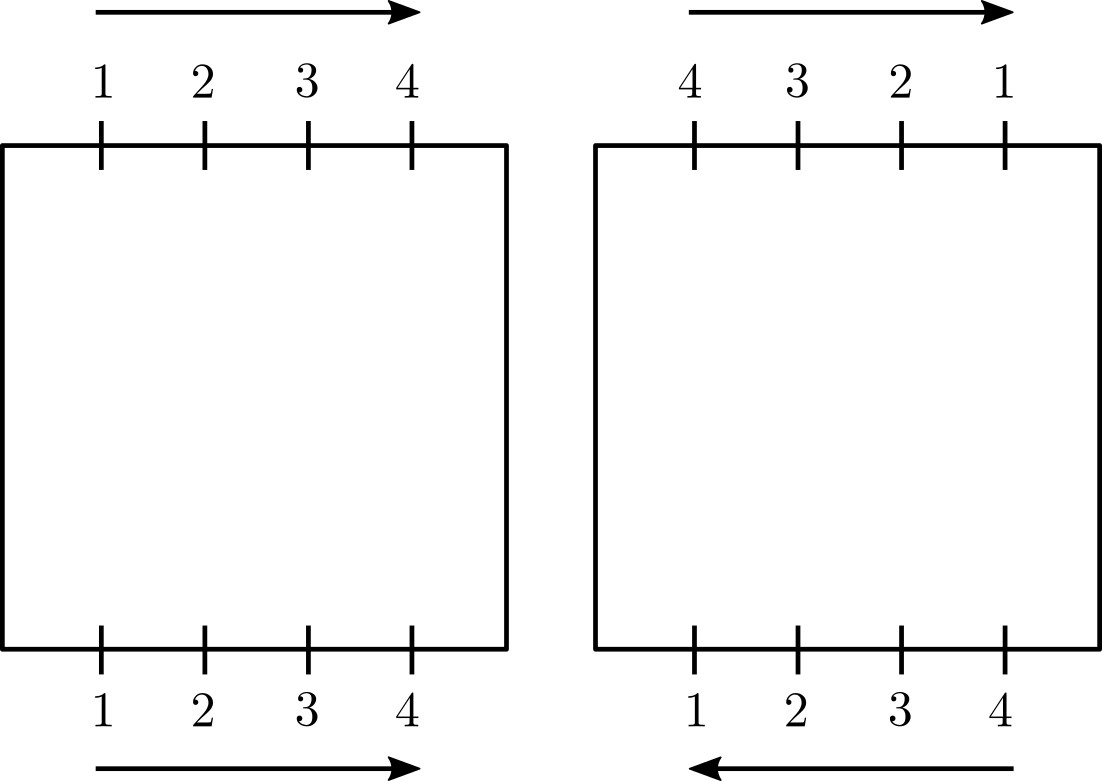
\includegraphics[width=6cm]{Img/GEO/geo-atlas1.jpg}
\centering
\caption{\footnotesize{Orientación conservadora (izquierda), se obtiene como resultado un cilindro. Orientación inversora (derecha), se obtiene una cinta de moebius \citep{Ramos2011}.}}
\label{fig:atlas0}
\end{figure}

Para especificar en el atlas de qué forma se van a unir las aristas, se utiliza la \textbf{paridad de transición} que es número $\pm 1$ (+ 1 si es conservadora, -1 si es inversora), unido al par de aristas. La figura \ref{fig:atlas1} presenta tres ejemplos de esta notación.

\begin{figure}[h]
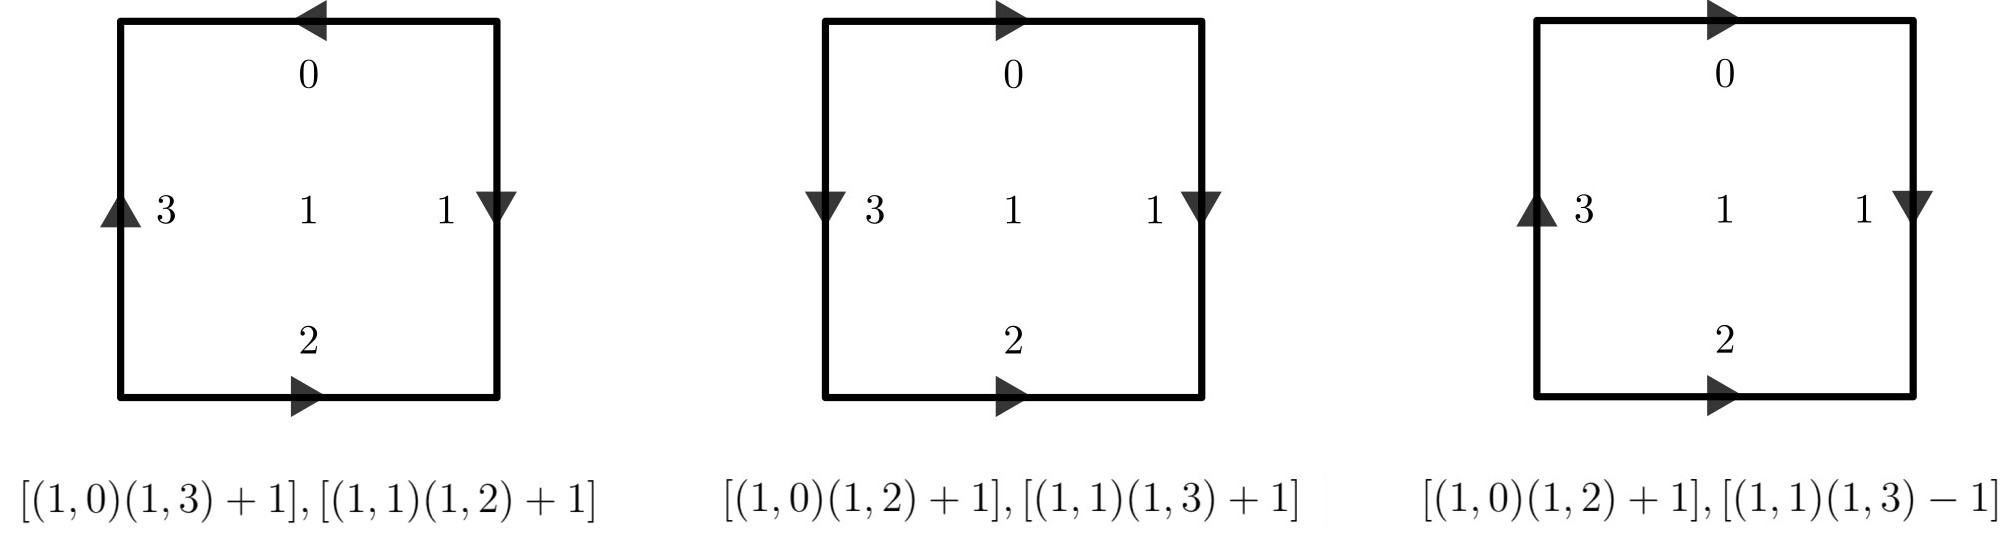
\includegraphics[width=15cm]{Img/GEO/atlas3.jpg}
\centering
\caption{\footnotesize{Paridad de transición de una. Esfera (izquierda). Toro (centro). Botella de Klein (izquierda), se puede observar la paridad de transición $-1$ \citep{Ramos2011}.}}
\label{fig:atlas1}
\end{figure}

\vspace{5mm}
Si se utilizan uniones no conservadoras en un atlas se consiguen algunas curiosidades matemáticas llamadas \textbf{superficies no orientables}, como la \textbf{cinta de Moebius} y la \textbf{botella de Klein}\footnote{En topología, una botella de Klein es una superficie no orientable abierta cuya característica de Euler es igual a $0$; no tiene interior ni exterior.} (ver figura \ref{fig:atlas2}). La cinta de Moebius posee una curiosa particularidad. Si se recorre la cinta comenzando en un punto cualquiera, y se da una vuelta completa, como se trata de una cinta bidimensional, cuando se llegue al punto de partida se observará que la derecha e izquierda están intercambiadas. 
Si se parte de una cinta de Moebius y se cierra aplicando una orientación conservadora, se obtiene una botella de Klein (no orientable), que no se puede construir en un espacio tridimensional sin que se auto interseque.
Este tipo de superficies se llaman \textbf{no orientables} y se producen al efectuar uniones no conservadoras entre sus aristas. Por el contrario, si en la superficie nunca se intercambian la izquierda y derecha, entonces se dice que la superficie es \textbf{orientable}.

\begin{figure}[h]
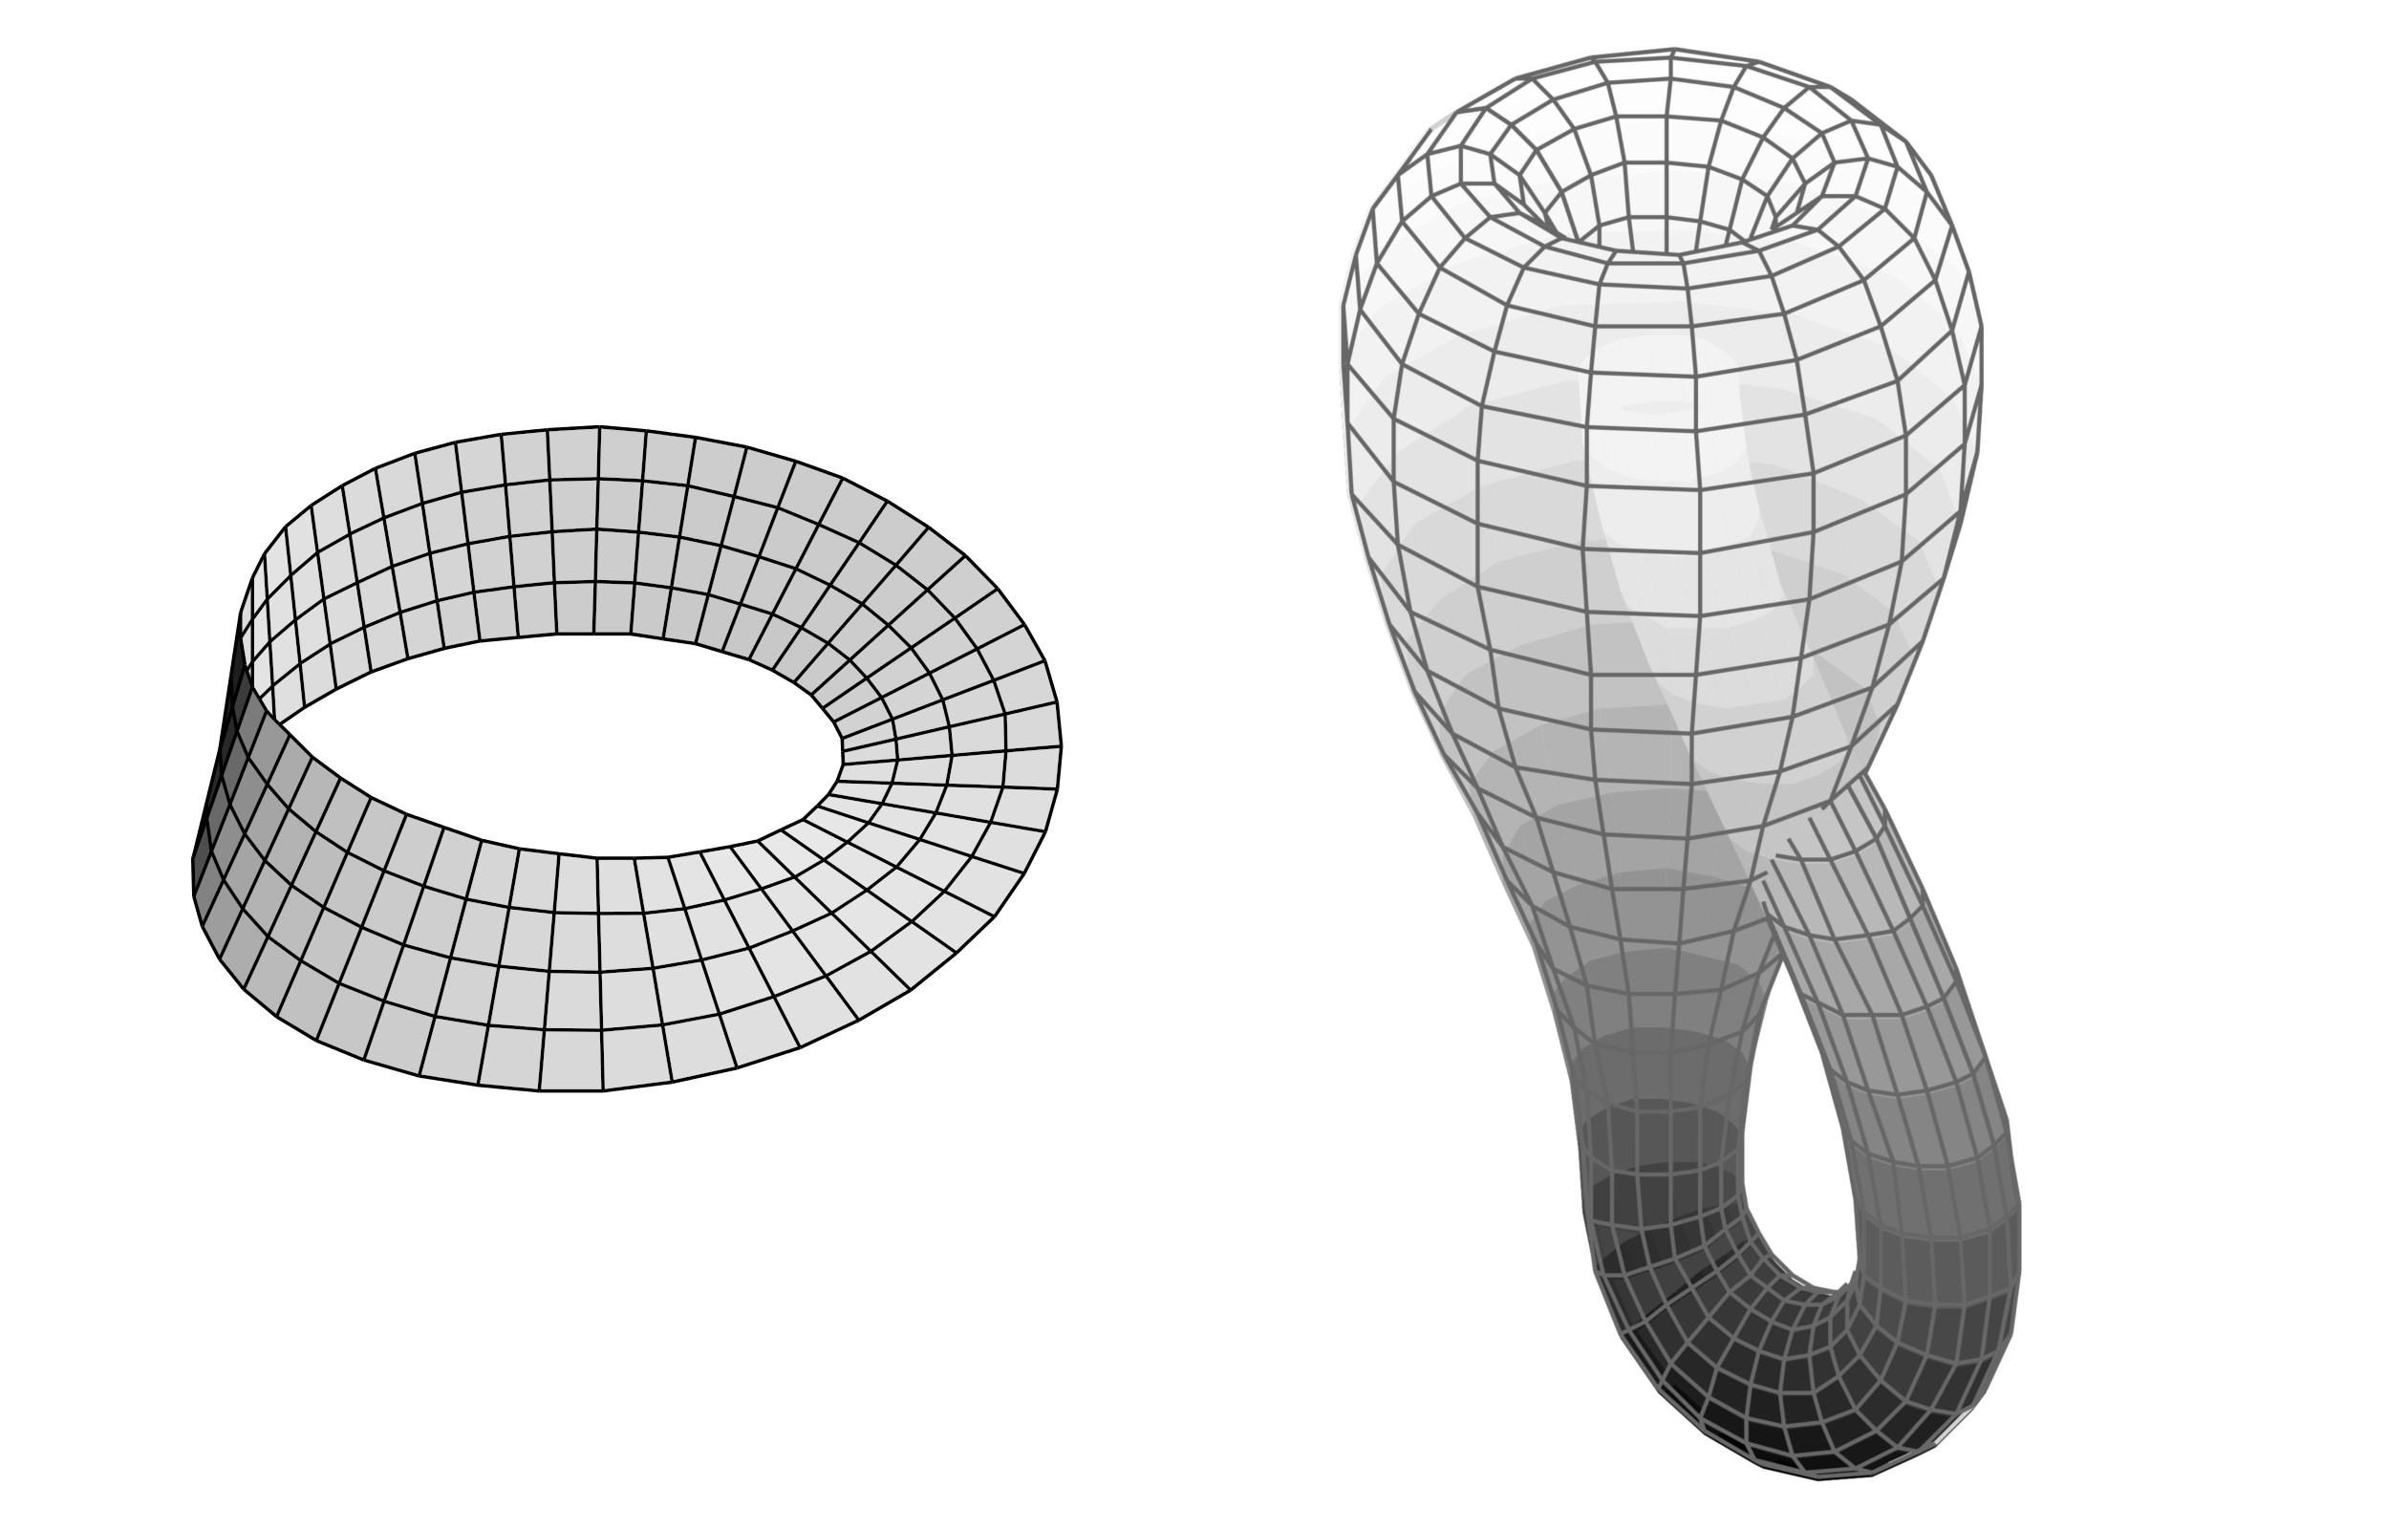
\includegraphics[width=10cm]{Img/GEO/geo-mobius.jpg}
\centering
\caption{\textbf{\footnotesize{Superficies no orientables. Cinta de Moebius (izquierda) y Botella de Klein (derecha) \citep{Ramos2011}.}}}
\label{fig:atlas2}
\end{figure}

\textquote{\textit{%Habíamos visto que 
Para que cualquier superficie cerrada tridimensional sea consistente, debe ser topológicamente equivalente a una esfera con ``$g$'' asas. Ahora se añade otra condición más: \textbf{debe ser orientable}}} \citep{Ramos2011}.\newline



\subsubsection{Representación mediante operadores Booleanos. }

Para construir objetos sólidos complejos se pueden utilizar operaciones entre conjuntos, tales como unión $(\cup)$, intersección $(\cap)$ y diferencia ($-$). A estos operadores se les conoce en modelado como \textbf{Operadores Booleanos} \citep{Ramos2011}. Al aplicarlos sobre objetos simples se pueden construir modelos más complejos. Es fundamental que los modelos obtenidos sean íntegros (topológicamente válidos), y que además sean \textbf{dimensionalmente homogéneos}, es decir, que su dimensión sea igual a la de los objetos que se combinan. En la figura \ref{fig:booleano1} se pueden apreciar los resultados de las operaciones booleanas entre una esfera y un cubo.

\begin{figure}[ht]
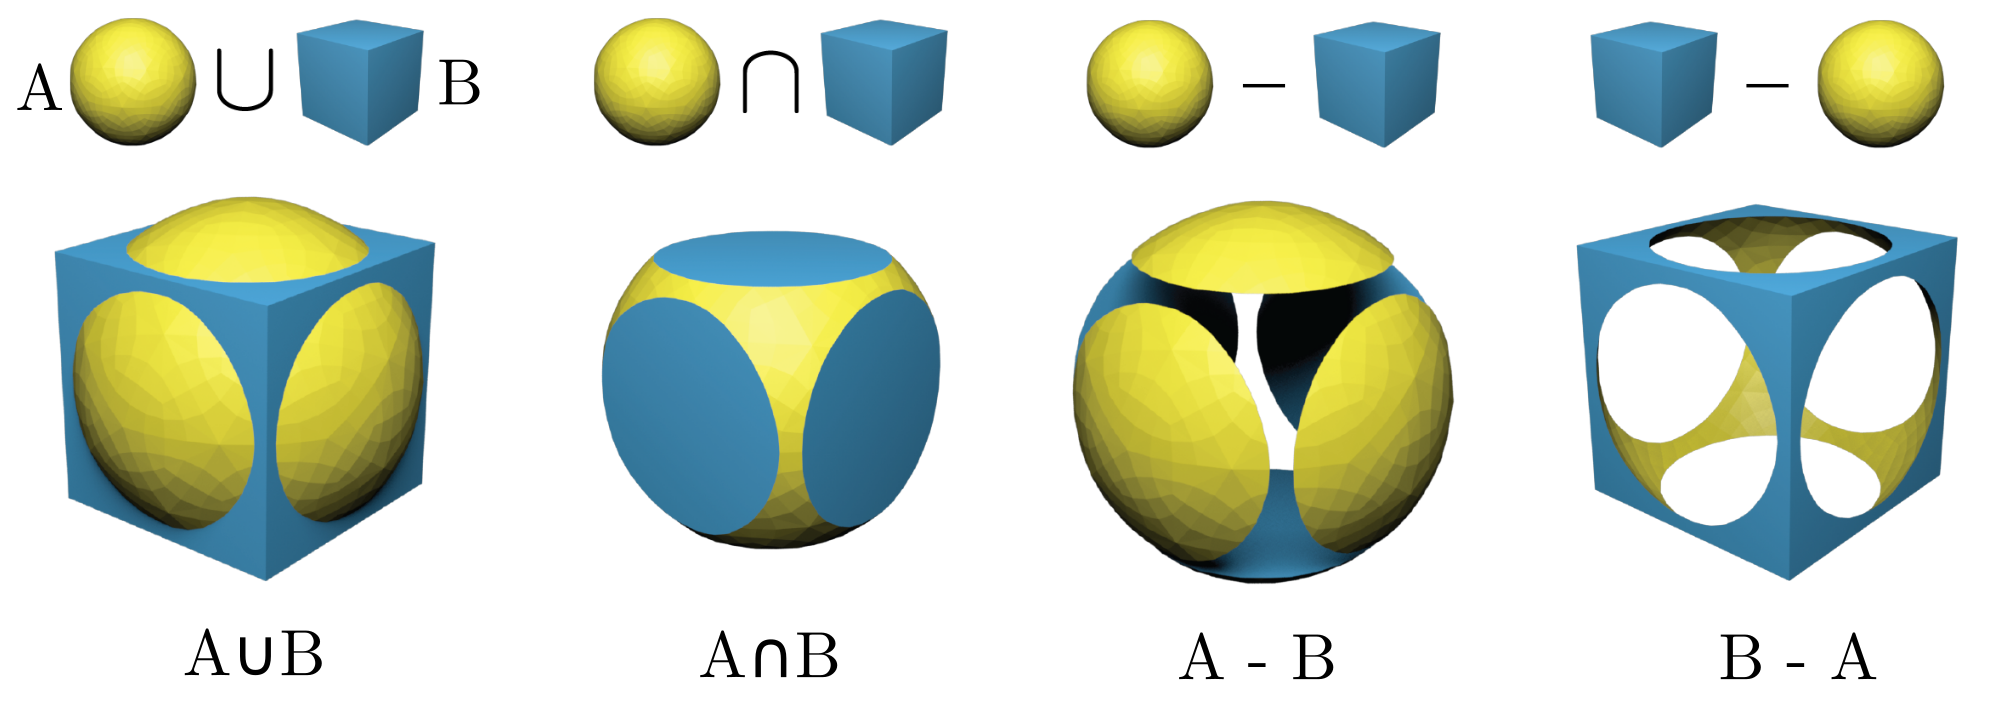
\includegraphics[width=10cm]{Img/GEO/boolean55.png}
\centering
\caption{\footnotesize{Operaciones booleanas entre objetos A(esfera) y B(cubo). Resultados de $A \cup B$,  $A \cap B$, $A - B$  y  $B - A$ } respectivamente \citep{Zhou2018}.}
\label{fig:booleano1}
\end{figure}

\vspace{5mm}

Sin embargo, la aplicación de una operación booleana a objetos sólidos no necesariamente produce otro objeto sólido. En la figura \ref{solucion-solido} se muestra un ejemplo donde se pierde la homogeneidad dimensional. Para evitar los resultados no sólidos se utiliza el conjunto de \textbf{operadores regularizados} \citep{Ramos2011}, que preservan la homogeneidad dimensional. Los operadores regularizados se representan por $\cup^*$, $\cap^*$ y $-^*$ y se definen de manera que las operaciones con sólidos siempre generen sólidos. 

\begin{figure}[ht]
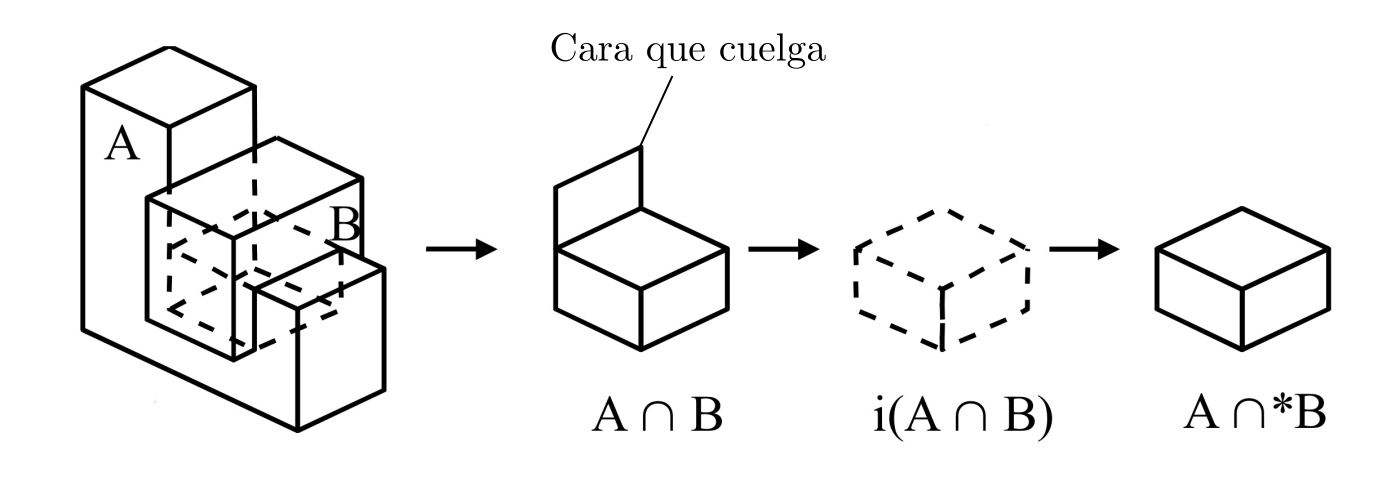
\includegraphics[width=11cm]{Img/GEO/geo-booleano2.png}
\centering
\caption{\footnotesize{Intersección no regularizada ($\cap$) y regularizada ($\cap^*$) de dos sólidos. La intersección $A (\cap) B$ entre dos objetos válidos 3D obtiene como resultado un objeto con una cara que cuelga 2D. Luego se efectúan una serie de operaciones matemáticas $i(A (\cap) B)$ de manera que eliminen los componentes 2D, 1D. La intersección ordinaria se reemplaza por la intersección regularizada ($ A \cap^* B$) \citep{Torres2014} asegurando que siempre se generen objetos sólidos.}}
\label{solucion-solido}
\end{figure}


\subsection{Visualización}
\label{visGeo}

Un elemento indispensable para visualizar modelos 3D en una pantalla es la \textbf{Síntesis de imágenes}, definida como un \textquote{\textit{campo de la informática gráfica que se dedica principalmente al estudio y desarrollo de procesos para sintetizar imágenes raster}} \citet{Ramos2011}. 
Las computadoras deben realizar un conjunto de operaciones elementales  para conseguir pasar de la \textbf{representación de un modelo geométrico} tridimensional a su imagen plana en pantalla (2D), pero que para la impresión del observador parezca estar contemplando un sistema de visualización en el mundo real en 3D. 
Esquemáticamente, el objetivo principal de un sistema gráfico\footnote{Sistema gráfico se refiere al conjunto de programas y herramientas auxiliares que permiten la síntesis de imágenes raster, a partir de un modelo vectorial 3D.} se resume en la figura \ref{fig:grafica3}: la visualización o \textbf{rendering} se produce en función de las condiciones establecidas por el observador, cámara o visor $f(visor)$. Es necesario el visor para generar una imagen bidimensional discreta (raster) a partir de un espacio vectorial 3D, lo implica que no se puede mostrar simultáneamente en  pantalla toda la información del modelo sino solamente lo que alcanza a ver el observador.\newline


\begin{figure}[ht]
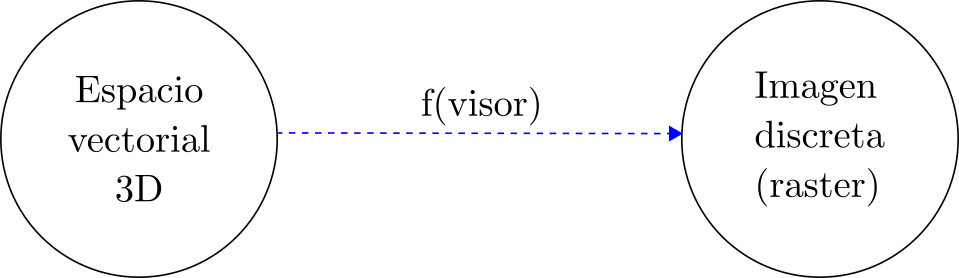
\includegraphics[width=8cm]{Img/CPD/grafica3.png}
\centering
\caption{\footnotesize{Esquema de visualización, se genera una imagen 2D (raster) a partir de un espacio vectorial 3D en función del visor $f(visor)$ \citep{Ramos2011}.}}
\label{fig:grafica3}
\end{figure}


La visualización se logra mediante una secuencia de operaciones conocida como \textit{viewing pipeline} \citep{marsh2005applied} ilustrada en la figura \ref{fig:view0}. 

\begin{figure}[ht]
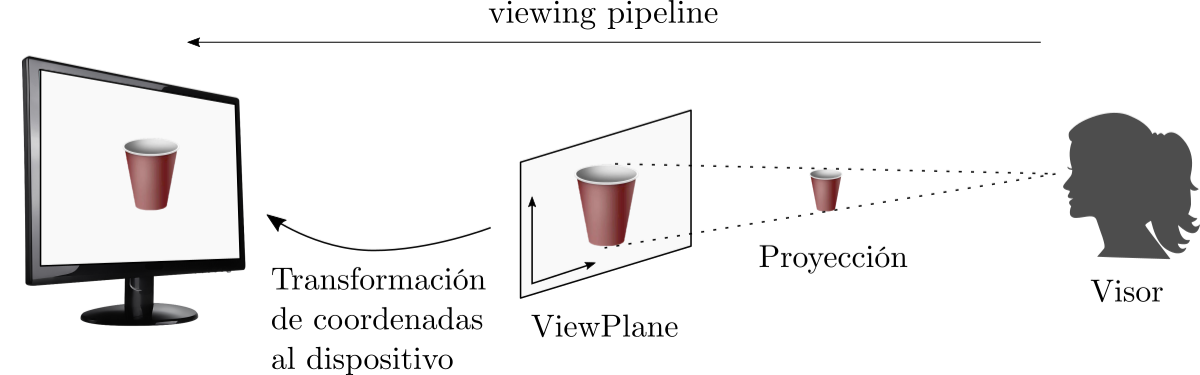
\includegraphics[width=13cm]{Img/GEO/geo-view001.png}
\centering
\caption{\footnotesize{Secuencia de operaciones para la visualización (viewing pipeline). En primer lugar, se aplica una proyección que mapea el objeto 3D a un nuevo objeto ``plano'' en un \textbf{plano de visión} en inglés \textit{Viewplain}.
Luego, se define un sistema de coordenadas en el viewplane especificando un punto como origen, y dos vectores perpendiculares que dan las direcciones de los ejes de coordenadas. Se aplica una asignación de coordenadas del viewplane para expresar el objeto ``plano'' en términos del sistema de coordenadas del plano bidimensional elegido. Finalmente, el objeto ``plano'' se asigna a la pantalla del dispositivo por medio de una transformación de coordenadas bidimensional \citep{marsh2005applied}.}}
\label{fig:view0}
\end{figure}


Básicamente hay dos métodos para proyectar objetos tridimensionales sobre una superficie bidimensional:  \textbf{proyección en perspectiva} y \textbf{proyección en paralelo}. 

Sea $n$ el vector plano de un viewplane, y sea $V$ (punto de visión o cámara) un punto que no está sobre el viewplane. La proyección en perspectiva de $V$ sobre $n$ es la transformación que mapea cualquier punto $P$ del objeto, distinto de $V$, en el punto $P^{\prime}$ que es la intersección de la línea $\overline{VP}$ y el plano $n$, como se ilustra en figura \ref{geo-view1} (a). La proyección se efectúa mediante líneas que convergen en una posición determinada. Si $V$ es un punto en el infinito, la proyección es paralela, todos los puntos del objeto se proyectan sobre la superficie bidimensional mediante líneas paralelas como se ilustra en la derecha de la figura figura \ref{geo-view1} (b).

\begin{figure}[h]
    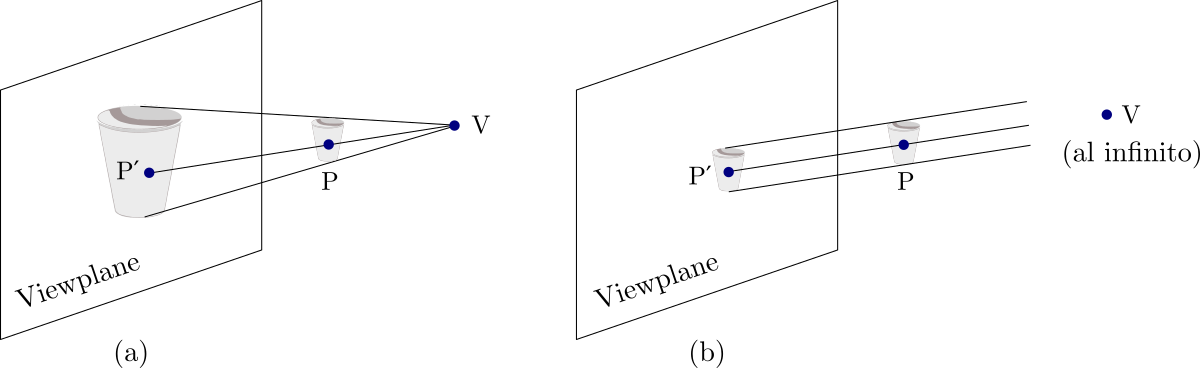
\includegraphics[width=14cm]{Img/GEO/geo-view11.png}
    \centering
    \caption{\footnotesize{a) proyección en perspectiva: La proyección del punto de visión $V$ es la transformación que mapea cualquier punto $P$ del objeto observado al punto $P^{\prime}$ sobre el $viewplain$. La proyección se efectúa mediante líneas que convergen en una posición determinada.
    b) proyección en paralelo:  $V$ es un punto de visión en el infinito. Todos los puntos del objeto $P$ se proyectan  mediante líneas paralelas a los respectivos en $P^{\prime}$ sobre la superficie bidimensional $Viewplain$ \citep{marsh2005applied}.}}
    \label{geo-view1}
\end{figure}

La proyección desde el punto de visión $V$ al viewplane $n$ es una transformación tridimensional dada por la matriz \citep{marsh2005applied}:

\begin{equation}
M = n^TV - (n  · V)I_4
\end{equation}

Siendo $I_4$ una matriz identidad 4x4.

\vspace{5mm}

Las tecnologías de visualización implementan estos conceptos de diferentes maneras dependiendo del contexto en que se utilizan, por ejemplo, en OpenGL\footnote{\url{https://www.opengl.org/}} se implementa la visualización mediante las matrices Modelo, Vista y Proyección en inglés \textit{model-view-projection matrix} \citep{kessenich2016opengl}.

En el diseño CAD es fundamental que los modelos estén bien definidos (consistentes) y la visualización es auxiliar (aunque necesaria), por lo que no tiene demasiada importancia la resolución\footnote{La resolución de una imagen indica la cantidad de detalles que puede observarse en esta. } de las imágenes, al menos en las primeras fases de diseño.\newline




\subsection{Diseño de Objetos} 
\label{sectionDisenoObjetos}
\label{disGeo}

Los modelos sólidos se pueden diseñar mediante el \textbf{modelado poligonal} \citep{russo2010polygonal} que consta en la manipulación de vértices, aristas o caras de los poliedros. Este enfoque es muy  flexible porque los ordenadores pueden renderizar los modelos muy rápido, sin embargo, al contener polígonos planos se dificulta la cobertura geométrica al construir modelos de geometría compleja, por ejemplo: para generar superficies curvas precisas se necesitan grandes cantidades de polígonos. Para solventar ese problema se utilizan otras técnicas de modelado, incluyendo:

\subsubsection{Modelado Booleano (CSG) }
\label{mod:booleano}
Al conjunto de procesos que permiten el diseño de sólidos complejos mediante la combinación booleana de objetos simples (primitivas) se conoce como \textbf{modelado booleano}, o también  \textbf{Geometría Constructiva de Sólidos} en inglés \textit{Constructive Solid Geometry} (CSG) \citep{foley1996computer}.\newline
En el modelado booleano, luego de escalar, trasladar y rotar convenientemente las primitivas, se aplican los operadores booleanos regularizados  ($\cup^*$, $\cap^*$ y $-^*$) para combinarlas. Un sólido construido mediante un modelador booleano (CSG) queda descrito mediante un árbol binario en el que:

\begin{itemize}
\item El nodo raíz es el sólido resultante.
\item Los nodos internos son los operadores booleanos.
\item Los nodos hoja son las primitivas.
\end{itemize}

En los nodos terminales del árbol no sólo se representan las primitivas, sino que también se indican las transformaciones lineales que se han de efectuar sobre ellas. En el árbol, tanto las operaciones como los nodos hoja deberán encontrarse ordenadas, debido a que las operaciones booleanas no son, en general, conmutativas. El proceso de seguimiento (recorrido) del árbol se hará partiendo de los nodos terminales.

\begin{figure}[ht]
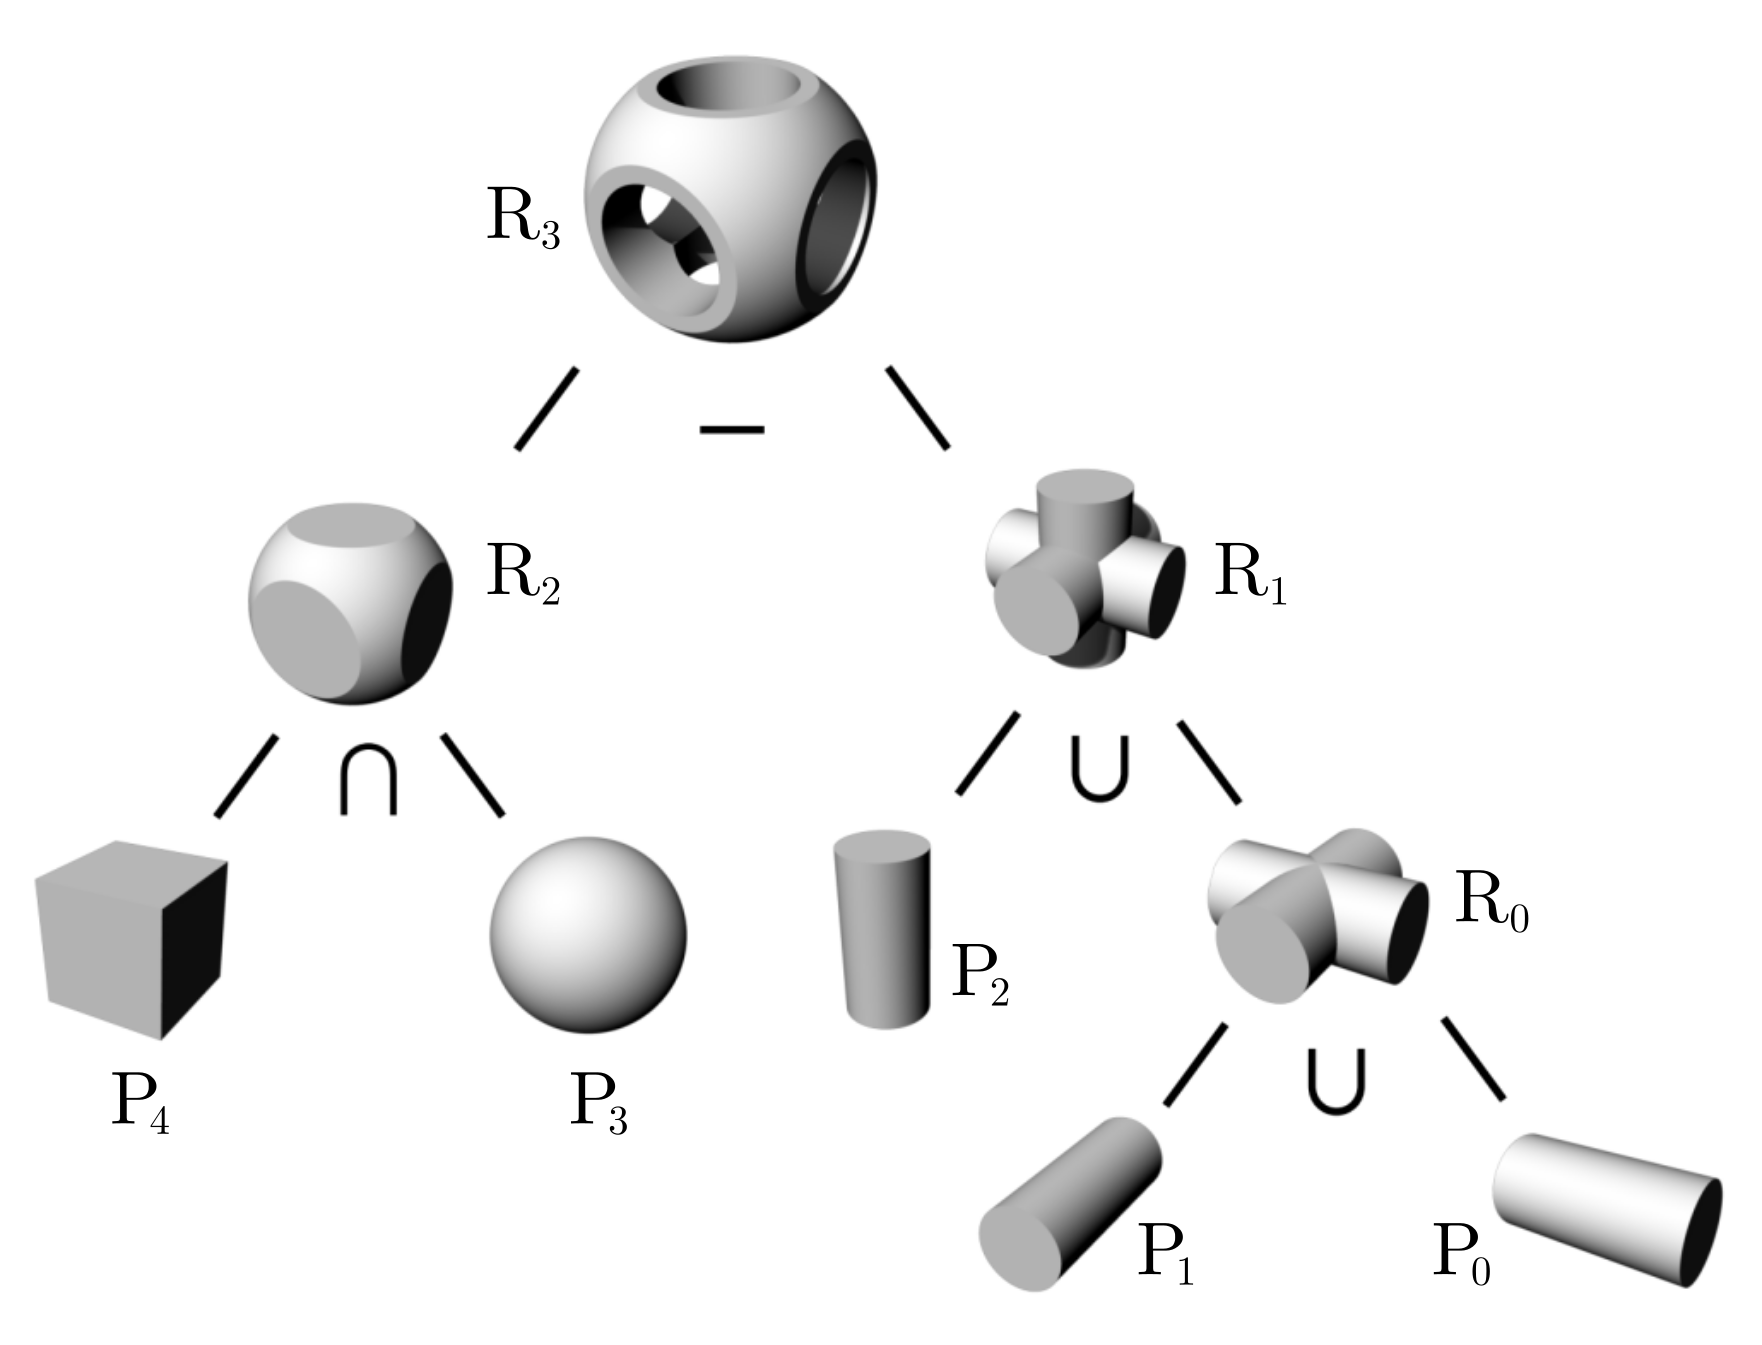
\includegraphics[width=10cm]{Img/GEO/geo-booleano6.png}
\centering
\caption{\footnotesize{Árbol CSG utilizando las   operaciones booleanas: unión ($\cup$), intersección ($\cap$) y diferencia ($-$). En la derecha se observa que $R_0$ es la unión de los cilindros $P_0$ y $P_1$ mediante la ecuación ($R_0 = P_0\cdot T_0 \cup P_1\cdot T_1$), luego se efectúa la unión entre $R_0$ y el cilindro $P_2$ dando como resultado $R_1$ mediante ($R_1 = R_0 \cup P_2\cdot T_2$). Por su parte en la izquierda $R_2$ es la intersección entre la esfera $P_3$ y el cubo $P_4$ $R_2 = P_3\cdot T_3 \cap P_4\cdot T_4$. Finalmente el nodo raíz resultante $R_3$ es la diferencia entre $R_2$ y $R_1$ mediante ($R_3 = R_2 - R_1$). También se aprecia un transformación de escala en la figura resultante, aumentando su tamaño, esto se debe a la aplicación de las matrices de transformación $T$ en cada operación \citep{Wassermann_2016}.}}
\label{fig:bool}
\end{figure}

En el ejemplo de la figura \ref{fig:bool} se puede ver la descripción de un modelo booleano, llamado R3.\newline Partiendo de las primitivas $P_0$ (cilindro), $P_1$ (cilindro), $P_2$ (cilindro), $P_3$ (esfera) y $P_4$ (cubo) se obtiene el objeto final ($R_3$) después de tres niveles de operaciones booleanas.\newline
En primer lugar se efectúa la unión de $P_0$ y $P_1$, después de haber transformado y posicionado adecuadamente las primitivas en el espacio, mediante las matrices netas $T_0$ y $T_1$.

\begin{equation}
R_0 = P_0\cdot T_0 \cup P_1\cdot T_1
\end{equation}

A continuación el resultado intermedio $R_0$ se suma con la primitiva $P_2$ (cilindro), después de haber sido escalada y posicionada por $T_2$.

\begin{equation}
R_1 = R_0 \cup P_2\cdot T_2
\end{equation}

Para producir el resultado $R_2$ se realiza la intersección entre $P_3$ y $P_4$, después de haber transformado y posicionado adecuadamente las primitivas en el espacio, mediante las matrices netas $T_3$ y $T_4$

\begin{equation}
R_2 = P_3\cdot T_3 \cap P_4\cdot T_4
\end{equation}

Finalmente, a $R_2$ se le resta $R_1$, obteniendo así el objeto raíz del árbol $R_3$.


\begin{equation}
R_3 = R_2 - R_1 = (P_3\cdot T_3 \cap P_4\cdot T_4) - ((P_0\cdot T_0 \cup P_1\cdot T_1) \cup (P_2\cdot T_2))
\end{equation}

En el ejemplo se puede apreciar que las transformaciones han incrementado el tamaño del sólido resultante $R_3$. Por lo general, el escalado de las primitivas no es uniforme, es decir, los factores de escala $s_x$, $s_y$, y $s_z$ son diferentes. De este modo, una sola primitiva puede proporcionar una gran variedad de copias diferentes simplemente usando transformaciones. \newline
Es importante indicar que el modelado booleano es un proceso descriptivo, es decir, sólo se limita a especificar qué primitivas se utilizan y cómo se combinan. De manera que sólo se dispone de la información geométrica y topológica de las primitivas pero no la de los objetos resultantes. Para poder combinar las primitivas en un esquema de modelado, éstas han de ser definidas previamente. Una forma frecuente de crearlas es estableciendo los parámetros de las ecuaciones que las definen. 


%\clearpage
\subsubsection{Diseño de nuevas primitivas}
La figura \ref{fig:csg3} muestra dos primitivas con los parámetros de control que cada una requiere (excluidos los de posición y orientación). Cuanto más flexible es esta definición, mayor es la capacidad para modelar los diferentes objetos y por consecuencia mayores son las posibilidades de modelado.\newline
Se llama dominio o \textbf{poder expresivo} de un modelador, a la capacidad que posee para modelar los diferentes objetos. Cuanto mayor sea el poder expresivo de un modelador, mayores son las posibilidades de modelado. 

\begin{figure}[ht]
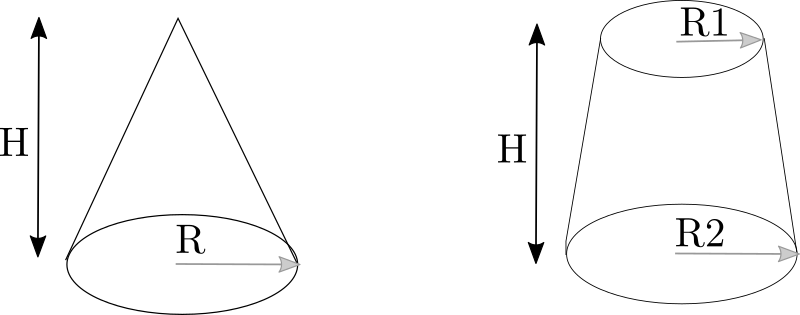
\includegraphics[width=6cm]{Img/GEO/geo-cono.png}
\centering
\caption{\footnotesize{Primitivas con sus parámetros de control. A la izquierda un cono con 2 parámetros: altura ($H$) y radio ($R$). A la derecha un cono truncado con 3 parámetros: altura ($H$), radio superior ($R1$) y radio inferior ($R2$). La primitiva de la izquierda en 3D solo puede generar conos. La primitiva de la  derecha por su parte puede generar cilindros, conos y conos truncados. Por ende, el poder expresivo de esta última es superior.
\citep{Ramos2011}.}}
\label{fig:csg3}
\end{figure}


Un sistema de modelado debería permitir al usuario definir sus propias primitivas y así aumentar el dominio y/o la potencia del modelador. En la generación de nuevos ejemplares, el sistema define un conjunto objetos sólidos que son relevantes para el área de aplicación. Estas primitivas suelen parametrizarse no sólo en función de las transformaciones, sino también con base a otras propiedades. Por ejemplo, objetos como engranajes o tuercas son tediosos de definir utilizando combinaciones booleanas de objetos más sencillos pero pueden ser formulados fácilmente con parámetros de alto nivel como diámetro, espesor, número de dientes, etc. (Ver figura \ref{fig:csg4}). 


\newline


\begin{figure}[h]
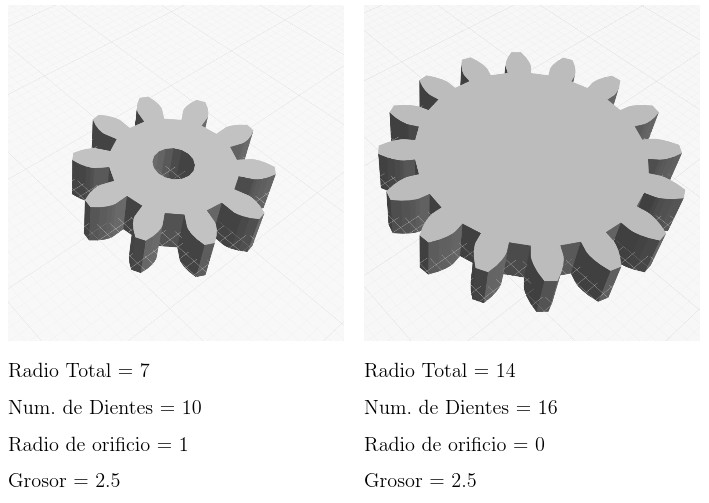
\includegraphics[width=12cm]{Img/Modelos/engranaje.jpg}
\centering
\caption{\footnotesize{Dos engranajes generados a partir de la misma primitiva. El cambio en los parámetros genera objetos con diferentes características. El engranaje de la derecha no posee ningún orificio, producto del cambio de valor $Radio \ de \ orificio = 0$}.}
\label{fig:csg4}
\end{figure}

La única forma de modelar un nuevo tipo de objeto es describiendo el mecanismo que lo define, es decir, es necesario escribir las rutinas o programas que lo dibujan o determinan sus propiedades.





\section{Sistemas CAD}
Para comprender el estado actual del CAD primero se deben estudiar algunas aplicaciones disponibles. 
Las soluciones presentadas incluyen herramientas basadas en el escritorio y basadas en la web. A continuación se describen las características más relevantes para este trabajo: Permitir el diseño paramétrico, contar con interfaz de scripting y proveer mecanismos para generar modelos sólidos.


\subsubsection{Blender} 
\textbf{Blender} \citep{BlenderFoundation} es una una suite de creación 3D FLOSS compatible con la totalidad del trabajo en 3D: modelado, rigging, animación, simulación, renderizado, composición y tracking de movimiento, incluso edición de video y creación de videojuegos. Esta aplicación esta principalmente está orientada a producciones artísticas, sin embargo, dispone de herramientas y primitivas para generar sólidos orientados a la fabricación digital. También permite el uso de modificadores que son operaciones automáticas que afectan a un objeto de una manera no destructiva\footnote{ No destructivo se refiere a hecho de realizar cambios sin sobrescribir los datos del modelo original, de manera que se puedan revertir.}. Con los modificadores, se pueden realizar tareas que manualmente serían demasiado tediosas. Entre muchos otros, se encuentra el modificador booleano que valga la redundancia se utiliza para  operaciones booleanas entre objetos. Otra capacidad de blender es el acceso a su API\footnote{\url{https://docs.blender.org/api/current/}} mediante scripting, utilizando el lenguaje de programación python\footnote{\url{https://www.python.org/}}.


\begin{figure}[h]
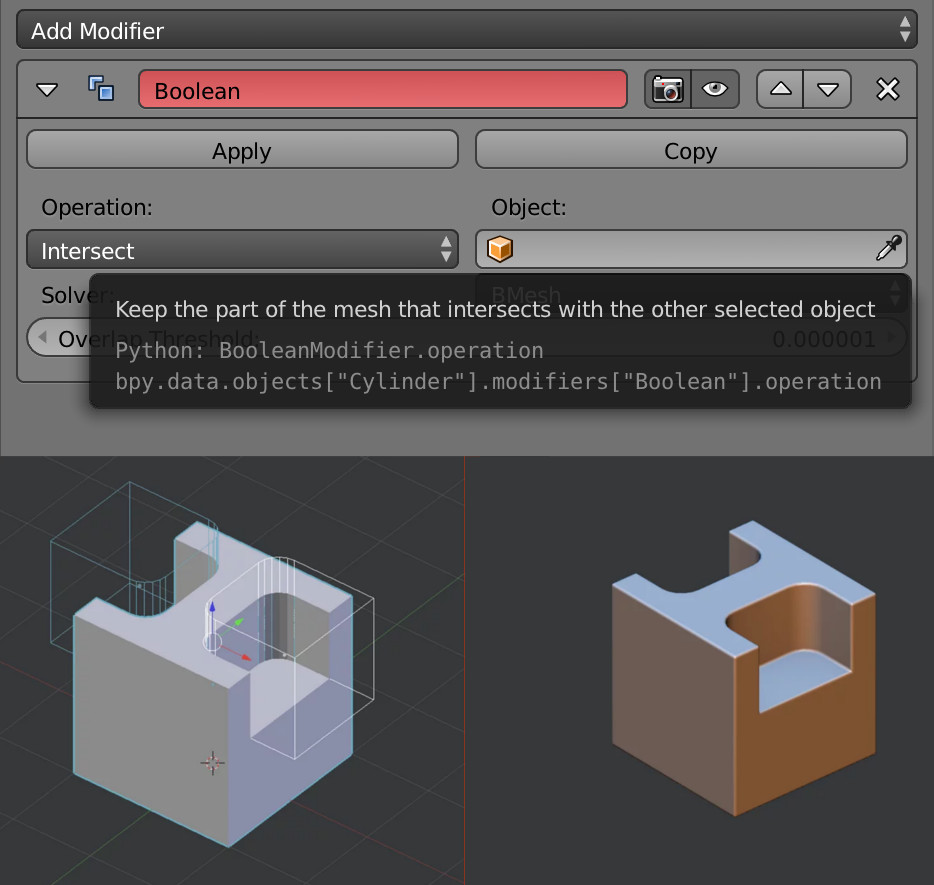
\includegraphics[width=8cm]{Img/Modelos/modelado22.jpg}
\centering
\caption{\footnotesize{Interfaz de Blender. Aplicación de intersecciones mediante el Modificador booleano. Se puede observar el código en python para realizar la operación mediante la API de Blender.  \citep{blenderBoolean}. }}
\end{figure}


\subsubsection{Grasshopper} 
En la última década se ha visto la aparición de un nuevo tipo de interfaz visual para scripting. Este tipo de programación visual implica representar programas no como texto, sino como diagramas. Un ejemplo de estas aplicaciones es \textbf{Grasshopper}  \citep{BobMcNeel}, un editor de algoritmos gráficos estrechamente integrado con las herramientas de modelado 3D de Rhino \footnote{\url{https://www.rhino3d.com/}}. Se basa principalmente en nodos que mapean el flujo de relaciones desde parámetros, a través de funciones definidas por el usuario, concluyendo normalmente con la generación de geometrías. Las modificaciones en los parámetros o las relaciones del modelo hacen que los cambios se propaguen a través de las funciones explícitas para volver a dibujar la geometría automáticamente. Esta es otra forma de crear modelos paramétricos.

\begin{figure}[h]
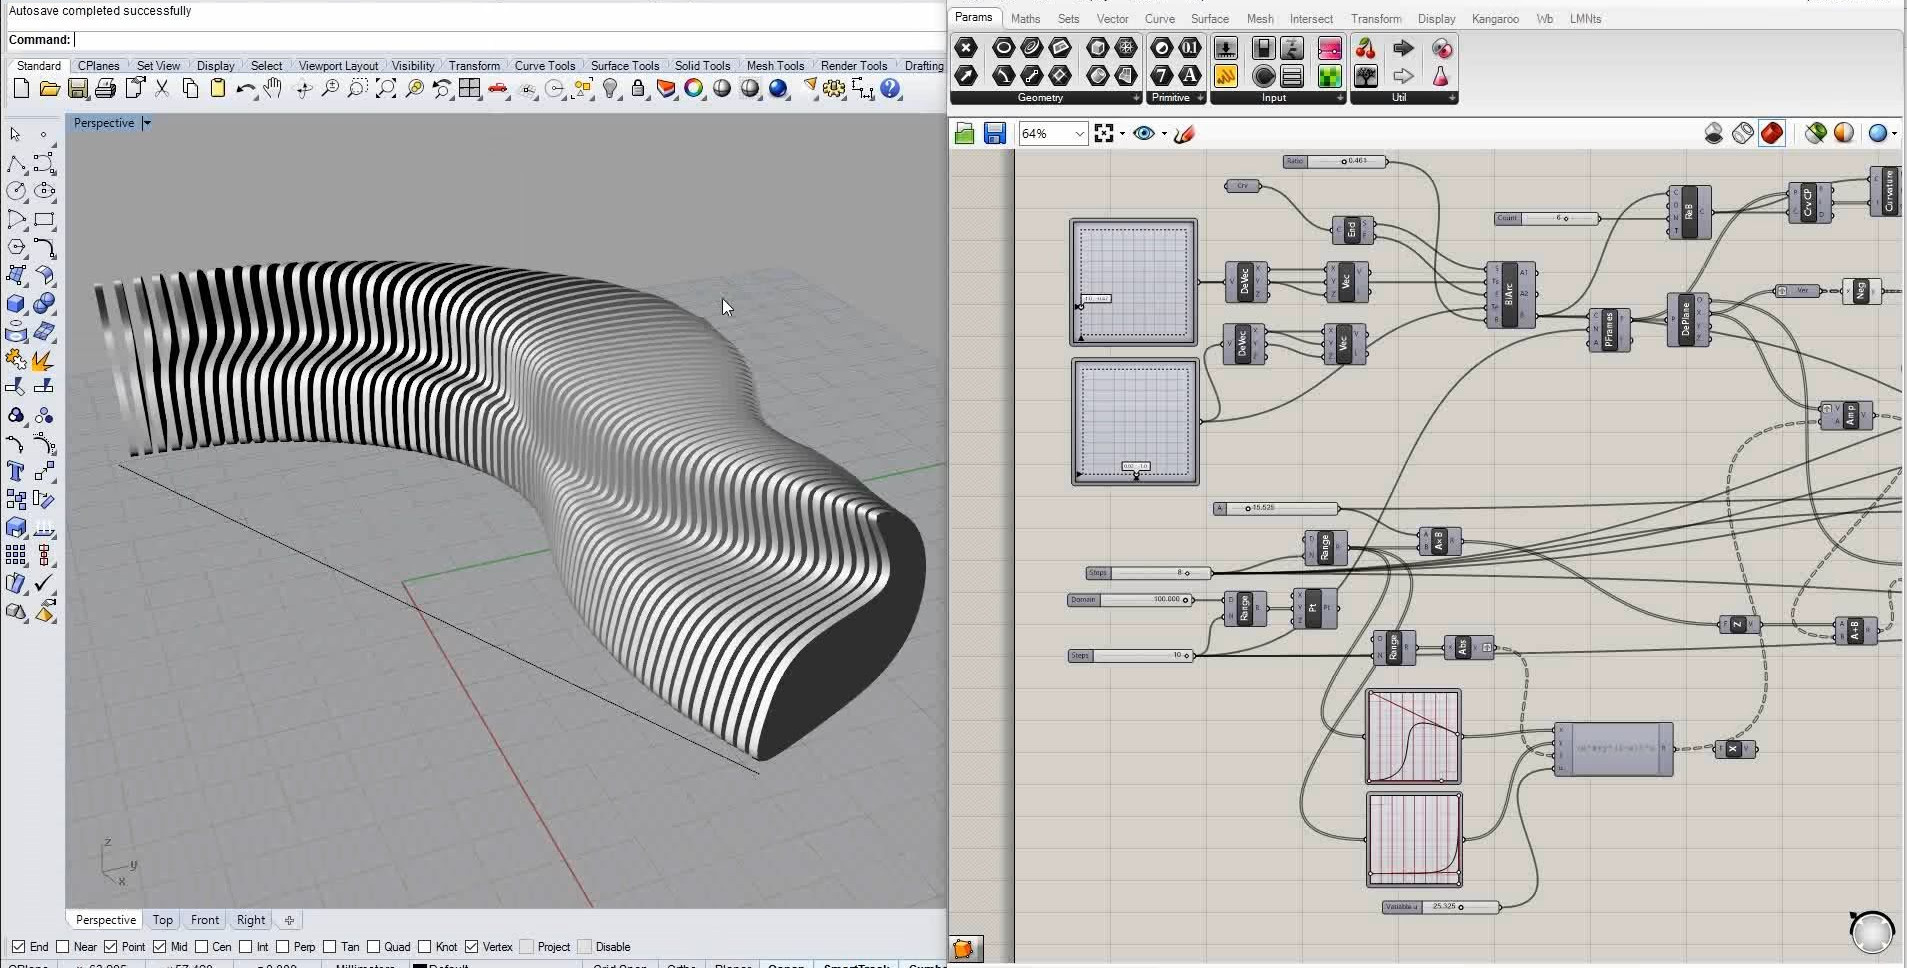
\includegraphics[width=14cm]{Img/CPD/cpd-grass.jpg}
\centering
\caption{\footnotesize{Programa en Grasshopper en forma de diagrama y las relaciones entre los nodos (derecha). Modelo resultante en la interfaz de Rhinoceros (derecha).  \citep{DanielParametric}.}}
\end{figure}


\subsubsection{OpenJSCAD} 
\textbf{OpenJSCAD}\footnote{\url{http://openjscad.org/}} está inspirado en OpenSCAD\footnote{\url{http://openscad.org/}} y esencialmente proporciona un enfoque a programadores para desarrollar modelos mediante una interfaz web. El diseño paramétrico se realiza mediante scripts en código javascript \citep{flanagan2007javascript} que utilizan funciones \textbf{CSG} y otras un tanto especiales, proporcionadas por el mismo entorno.
Permite incorporar parámetros en la interfaz gráfica, posibilitando al usuario cambiar los  valores de forma interactiva. OpenJSCAD utiliza otras librerías como base para cumplir con sus funcionalidades. Para modelado booleano requiere de \textbf{CSG.js} \footnote{\url{https://github.com/jscad/csg.js}} y para la visualización de los modelos 3D  utiliza \textbf{lightgl.js}  \footnote{\url{https://github.com/evanw/lightgl.js/}} que facilita el desarrollo de aplicaciones WebGL, re-implementando la matriz modelo-vista/proyección\footnote{\url{http://www.opengl-tutorial.org/es/beginners-tutorials/tutorial-3-matrices/}} (analizada en   la sección \ref{visGeo}) de OpenGL\footnote{\url{https://www.opengl.org/}} para proporcionar una funcionalidad similar. 

En la figura \ref{fig:openjscad} se puede ver a la izquierda el modelo 3D de un engranaje y los campos con sus parámetros. A la derecha se sitúa el editor de texto con el programa correspondiente escrito en javascript.

\begin{figure}[h]
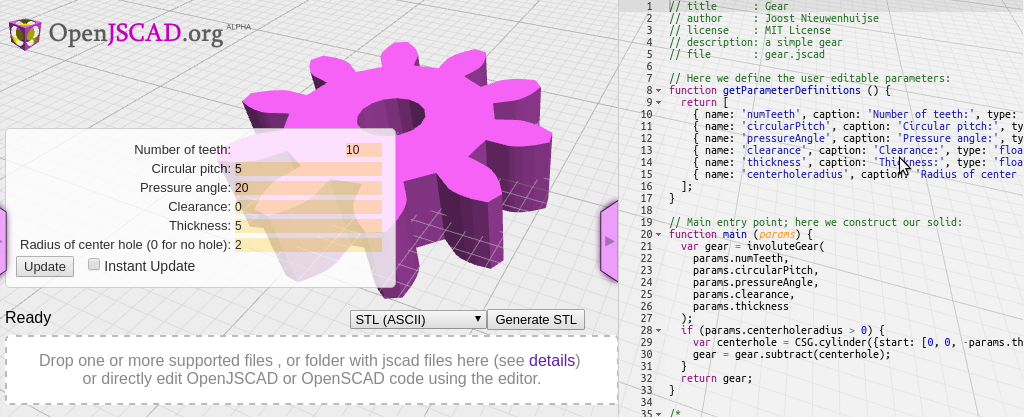
\includegraphics[width=14cm]{Img/openjscad-params.png}
\centering
\caption{\footnotesize{
Interfaz de OpenJSCAD. Modelo 3D de un engranaje y los campos con sus paŕametros  (izquierda) y la especificación del modelo mediante código javascript (derecha).
\citep{openJSCADorg}.}}
\label{fig:openjscad}
\end{figure}



\subsubsection{OnShape} 
\textbf{OnShape}\footnote{\url{https://www.onshape.com/}} es una aplicación CAD basada en la nube que puede ser accedida desde cualquier navegador o mediante su aplicación para móviles. Su dominio esta fuertemente orientado al \textbf{diseño mecánico} \citep{lardies2012criterios} con características similares a programas como SolidWorks\footnote{\url{https://www.solidworks.com/es}}. 
Cuenta con un sistema de control de versiones\footnote{Se llama control de versiones a la gestión de los diversos cambios que se realizan sobre los elementos de algún producto o una configuración del mismo} para los documentos del proyecto (dibujos, modelos 3d y documentos) y soporta la colaboración en tiempo real. La aproximación de modelado es de manipulación directa, sin embargo, incluye un lenguaje de scripting que se denomina FeatureScript\footnote{\url{https://cad.onshape.com/FsDoc/}} y permite la definición de la geometría, relaciones y parámetros para la construcción de modelos 3D Paramétricos \citep{Alfaiate2017}.

\begin{figure}[h]
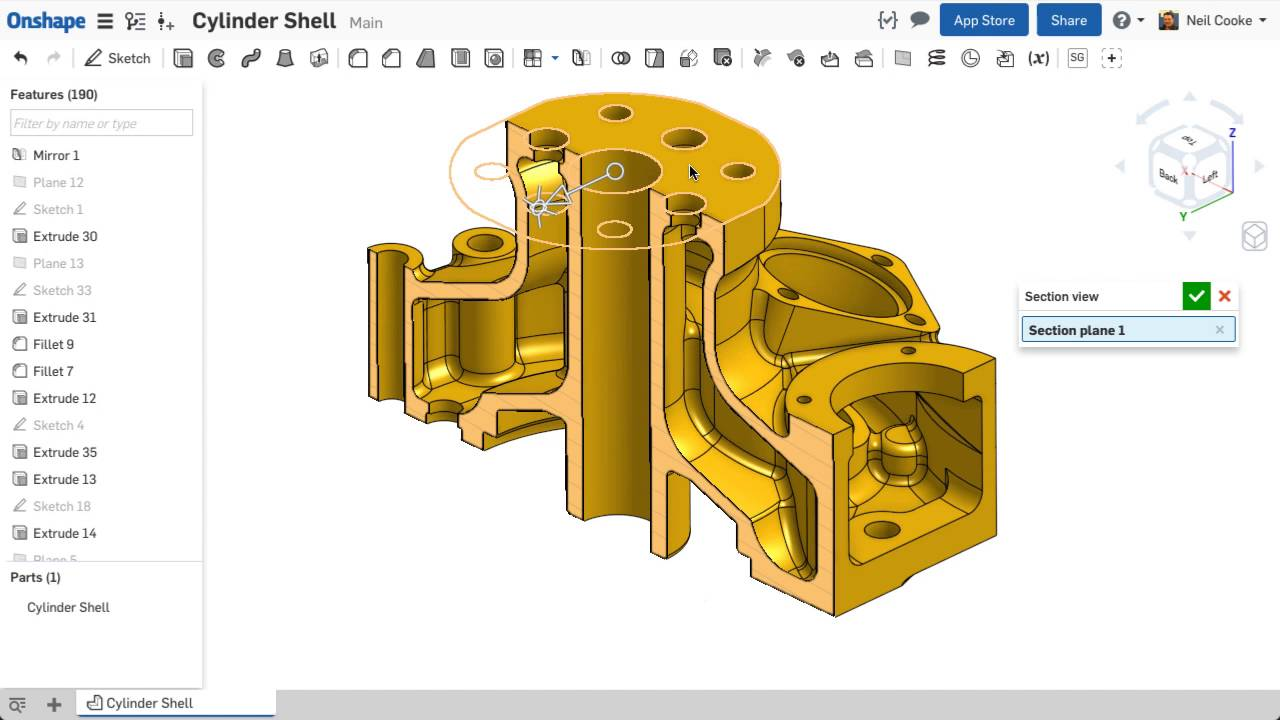
\includegraphics[width=14cm]{Img/onshape.jpg}
\centering
\caption{\footnotesize{Interfaz de OnShape con un modelo mecánico \citep{OnshapePlanes}.}}
\end{figure}
